%*************************************************************************
% A Classic Thesis Style
% An Homage to The Elements of Typographic Style
%
% Copyright (C) 2017 André Miede and Ivo Pletikosić
%
% If you like the style then I would appreciate a postcard. My address
% can be found in the file ClassicThesis.pdf. A collection of the
% postcards I received so far is available online at
% http://postcards.miede.de
%
% License:
% This program is free software; you can redistribute it and/or modify
% it under the terms of the GNU General Public License as published by
% the Free Software Foundation; either version 2 of the License, or
% (at your option) any later version.
%
% This program is distributed in the hope that it will be useful,
% but WITHOUT ANY WARRANTY; without even the implied warranty of
% MERCHANTABILITY or FITNESS FOR A PARTICULAR PURPOSE.  See the
% GNU General Public License for more details.
%
% You should have received a copy of the GNU General Public License
% along with this program; see the file COPYING.  If not, write to
% the Free Software Foundation, Inc., 59 Temple Place - Suite 330,
% Boston, MA 02111-1307, USA.
%
% PLEASE SEE ALSO THE AUTHORS' NOTE REGARDING THIS LICENSE
% IN THE DOCUMENTATION (ClassicThesis.pdf --> Chapter 1 / Chapter01.tex)
%*************************************************************************
\RequirePackage{silence} % :-\
    \WarningFilter{scrreprt}{Usage of package `titlesec'}
    %\WarningFilter{scrreprt}{Activating an ugly workaround}
    \WarningFilter{titlesec}{Non standard sectioning command detected}
\documentclass[ openright,titlepage,numbers=noenddot,headinclude,%twoside, %1headlines,% letterpaper a4paper
                footinclude=true,cleardoublepage=empty,
                BCOR=5mm,paper=a4,fontsize=11pt,%11pt,a4paper,%
                ngerman,american,%lockflag%
                ]{scrreprt}

%*************************************************************************
% Note: Make all your adjustments in here
%*************************************************************************
% ****************************************************************************************************
% hdathesis-config.tex 
% Use it at the beginning of your thesis.tex, or as a LaTeX Preamble 
% in your thesis.{tex,lyx} with % ****************************************************************************************************
% hdathesis-config.tex 
% Use it at the beginning of your thesis.tex, or as a LaTeX Preamble 
% in your thesis.{tex,lyx} with % ****************************************************************************************************
% hdathesis-config.tex 
% Use it at the beginning of your thesis.tex, or as a LaTeX Preamble 
% in your thesis.{tex,lyx} with \input{hdathesis-config}
% ****************************************************************************************************

% ****************************************************************************************************
% 1. Personal data and user ad-hoc commands
% ****************************************************************************************************
\newcommand{\myTitle}{SmartTrain: Autonomous Train Control System with Local LLM Integration\xspace}
%\newcommand{\mySubtitle}{An Homage to The Elements of Typographic Style\xspace}
%\newcommand{\myDegree}{Bachelor of Science (B.Sc.)\xspace} 
%\newcommand{\myDegree}{Bachelor of Arts (B.A.)\xspace}
\newcommand{\myDegree}{Master of Science (M.Sc.)\xspace}
%\newcommand{\myDegree}{Master of Arts (M.A.)\xspace}
\newcommand{\myName}{Indranil Ariunbold Behnke\xspace}
\newcommand{\myId}{745353\xspace}
\newcommand{\myProf}{Prof. Dr. Frank Bühler\xspace}
\newcommand{\myOtherProf}{Prof. Dr. Michael Massoth\xspace}
\newcommand{\myFaculty}{Fachbereich Informatik\xspace}
\newcommand{\myUni}{Hochschule Darmstadt\xspace}
\newcommand{\myLocation}{Darmstadt\xspace}
\newcommand{\myTime}{20. March 2025\xspace}
\newcommand{\myVersion}{version 4.4\xspace}

% ****************************************************************************************************
% 2. Is it a master thesis?
% ****************************************************************************************************
%\PassOptionsToPackage{master}{hdathesis} % uncomment if this is a master thesis 

% ****************************************************************************************************
% 3. Does the thesis have a lock flag?
% ****************************************************************************************************
%\PassOptionsToPackage{lockflag}{hdathesis} % uncomment if this thesis has a lock flag 

% ****************************************************************************************************
% 4. Loading some handy packages
% ****************************************************************************************************
% ****************************************************************************************************
% Packages with options that might require adjustments
% ****************************************************************************************************

%\PassOptionsToPackage{ngerman,american}{babel}   % change this to your language(s)
% Spanish languages need extra options in order to work with this template
%\PassOptionsToPackage{spanish,es-lcroman}{babel}
\usepackage{babel}


% ****************************************************************************************************

% ****************************************************************************************************
% 1. Personal data and user ad-hoc commands
% ****************************************************************************************************
\newcommand{\myTitle}{SmartTrain: Autonomous Train Control System with Local LLM Integration\xspace}
%\newcommand{\mySubtitle}{An Homage to The Elements of Typographic Style\xspace}
%\newcommand{\myDegree}{Bachelor of Science (B.Sc.)\xspace} 
%\newcommand{\myDegree}{Bachelor of Arts (B.A.)\xspace}
\newcommand{\myDegree}{Master of Science (M.Sc.)\xspace}
%\newcommand{\myDegree}{Master of Arts (M.A.)\xspace}
\newcommand{\myName}{Indranil Ariunbold Behnke\xspace}
\newcommand{\myId}{745353\xspace}
\newcommand{\myProf}{Prof. Dr. Frank Bühler\xspace}
\newcommand{\myOtherProf}{Prof. Dr. Michael Massoth\xspace}
\newcommand{\myFaculty}{Fachbereich Informatik\xspace}
\newcommand{\myUni}{Hochschule Darmstadt\xspace}
\newcommand{\myLocation}{Darmstadt\xspace}
\newcommand{\myTime}{20. March 2025\xspace}
\newcommand{\myVersion}{version 4.4\xspace}

% ****************************************************************************************************
% 2. Is it a master thesis?
% ****************************************************************************************************
%\PassOptionsToPackage{master}{hdathesis} % uncomment if this is a master thesis 

% ****************************************************************************************************
% 3. Does the thesis have a lock flag?
% ****************************************************************************************************
%\PassOptionsToPackage{lockflag}{hdathesis} % uncomment if this thesis has a lock flag 

% ****************************************************************************************************
% 4. Loading some handy packages
% ****************************************************************************************************
% ****************************************************************************************************
% Packages with options that might require adjustments
% ****************************************************************************************************

%\PassOptionsToPackage{ngerman,american}{babel}   % change this to your language(s)
% Spanish languages need extra options in order to work with this template
%\PassOptionsToPackage{spanish,es-lcroman}{babel}
\usepackage{babel}


% ****************************************************************************************************

% ****************************************************************************************************
% 1. Personal data and user ad-hoc commands
% ****************************************************************************************************
\newcommand{\myTitle}{SmartTrain: Autonomous Train Control System with Local LLM Integration\xspace}
%\newcommand{\mySubtitle}{An Homage to The Elements of Typographic Style\xspace}
%\newcommand{\myDegree}{Bachelor of Science (B.Sc.)\xspace} 
%\newcommand{\myDegree}{Bachelor of Arts (B.A.)\xspace}
\newcommand{\myDegree}{Master of Science (M.Sc.)\xspace}
%\newcommand{\myDegree}{Master of Arts (M.A.)\xspace}
\newcommand{\myName}{Indranil Ariunbold Behnke\xspace}
\newcommand{\myId}{745353\xspace}
\newcommand{\myProf}{Prof. Dr. Frank Bühler\xspace}
\newcommand{\myOtherProf}{Prof. Dr. Michael Massoth\xspace}
\newcommand{\myFaculty}{Fachbereich Informatik\xspace}
\newcommand{\myUni}{Hochschule Darmstadt\xspace}
\newcommand{\myLocation}{Darmstadt\xspace}
\newcommand{\myTime}{20. March 2025\xspace}
\newcommand{\myVersion}{version 4.4\xspace}

% ****************************************************************************************************
% 2. Is it a master thesis?
% ****************************************************************************************************
%\PassOptionsToPackage{master}{hdathesis} % uncomment if this is a master thesis 

% ****************************************************************************************************
% 3. Does the thesis have a lock flag?
% ****************************************************************************************************
%\PassOptionsToPackage{lockflag}{hdathesis} % uncomment if this thesis has a lock flag 

% ****************************************************************************************************
% 4. Loading some handy packages
% ****************************************************************************************************
% ****************************************************************************************************
% Packages with options that might require adjustments
% ****************************************************************************************************

%\PassOptionsToPackage{ngerman,american}{babel}   % change this to your language(s)
% Spanish languages need extra options in order to work with this template
%\PassOptionsToPackage{spanish,es-lcroman}{babel}
\usepackage{babel}


% ****************************************************************************************************
% classicthesis-config.tex
% formerly known as loadpackages.sty, classicthesis-ldpkg.sty, and classicthesis-preamble.sty
% Use it at the beginning of your ClassicThesis.tex, or as a LaTeX Preamble
% in your ClassicThesis.{tex,lyx} with % ****************************************************************************************************
% classicthesis-config.tex
% formerly known as loadpackages.sty, classicthesis-ldpkg.sty, and classicthesis-preamble.sty
% Use it at the beginning of your ClassicThesis.tex, or as a LaTeX Preamble
% in your ClassicThesis.{tex,lyx} with % ****************************************************************************************************
% classicthesis-config.tex
% formerly known as loadpackages.sty, classicthesis-ldpkg.sty, and classicthesis-preamble.sty
% Use it at the beginning of your ClassicThesis.tex, or as a LaTeX Preamble
% in your ClassicThesis.{tex,lyx} with \input{classicthesis-config}
% ****************************************************************************************************
% If you like the classicthesis, then I would appreciate a postcard.
% My address can be found in the file ClassicThesis.pdf. A collection
% of the postcards I received so far is available online at
% http://postcards.miede.de
% ****************************************************************************************************


% ****************************************************************************************************
% 0. Set the encoding of your files. UTF-8 is the only sensible encoding nowadays. If you can't read
% äöüßáéçèê∂åëæƒÏ€ then change the encoding setting in your editor, not the line below. If your editor
% does not support utf8 use another editor!
% ****************************************************************************************************
\PassOptionsToPackage{utf8}{inputenc}
  \usepackage{inputenc}

% ****************************************************************************************************
% 1. Configure classicthesis for your needs here, e.g., remove "drafting" below
% in order to deactivate the time-stamp on the pages
% (see ClassicThesis.pdf for more information):
% ****************************************************************************************************
\PassOptionsToPackage{
  drafting=false,   % print version information on the bottom of the pages
  tocaligned=false, % the left column of the toc will be aligned (no indentation)
  dottedtoc=true,   % page numbers in ToC flushed right
  parts=true,       % use part division
  eulerchapternumbers=true, % use AMS Euler for chapter font (otherwise Palatino)
  linedheaders=false,       % chaper headers will have line above and beneath
  floatperchapter=true,     % numbering per chapter for all floats (i.e., Figure 1.1)
  listings=true,    % load listings package and setup LoL
  subfig=true,      % setup for preloaded subfig package
  eulermath=false,  % use awesome Euler fonts for mathematical formulae (only with pdfLaTeX)
  beramono=true,    % toggle a nice monospaced font (w/ bold)
  minionpro=false   % setup for minion pro font; use minion pro small caps as well (only with pdfLaTeX)
}{classicthesis}


% ****************************************************************************************************
% 2. Personal data and user ad-hoc commands
% ****************************************************************************************************
%\newcommand{\myTitle}{A Classic Thesis Style\xspace}
%\newcommand{\mySubtitle}{An Homage to The Elements of Typographic Style\xspace}
%\newcommand{\myDegree}{Doktor-Ingenieur (Dr.-Ing.)\xspace}
%\newcommand{\myName}{André Miede\xspace}
%\newcommand{\myProf}{Put name here\xspace}
%\newcommand{\myOtherProf}{Put name here\xspace}
%\newcommand{\mySupervisor}{Put name here\xspace}
%\newcommand{\myFaculty}{Put data here\xspace}
%\newcommand{\myDepartment}{Put data here\xspace}
%\newcommand{\myUni}{Put data here\xspace}
%\newcommand{\myLocation}{Saarbrücken\xspace}
%\newcommand{\myTime}{October 2017\xspace}
%\newcommand{\myVersion}{version 4.4}

% ********************************************************************
% Setup, finetuning, and useful commands
% ********************************************************************
\newcounter{dummy} % necessary for correct hyperlinks (to index, bib, etc.)
\newlength{\abcd} % for ab..z string length calculation
\providecommand{\mLyX}{L\kern-.1667em\lower.25em\hbox{Y}\kern-.125emX\@}
\newcommand{\ie}{i.\,e.}
\newcommand{\Ie}{I.\,e.}
\newcommand{\eg}{e.\,g.}
\newcommand{\Eg}{E.\,g.}
% ****************************************************************************************************


% ****************************************************************************************************
% 3. Loading some handy packages
% ****************************************************************************************************
% ********************************************************************
% Packages with options that might require adjustments
% ********************************************************************
%\PassOptionsToPackage{ngerman,american}{babel}   % change this to your language(s), main language last
% Spanish languages need extra options in order to work with this template
%\PassOptionsToPackage{spanish,es-lcroman}{babel}
\usepackage{babel}

\usepackage{csquotes}

\PassOptionsToPackage{%
  %backend=biber,bibencoding=utf8, %instead of bibtex
  backend=bibtex8,bibencoding=ascii,%
  language=auto,%
  %style=numeric-comp,%
  style=alphabetic,%
  %style=authoryear-comp, % Author 1999, 2010
  %bibstyle=authoryear,dashed=false, % dashed: substitute rep. author with ---
  sorting=nyt, % name, year, title
  maxbibnames=10, % default: 3, et al.
  %backref=true,%
  natbib=true % natbib compatibility mode (\citep and \citet still work)
}{biblatex}
  \usepackage{biblatex}

\PassOptionsToPackage{fleqn}{amsmath}       % math environments and more by the AMS
  \usepackage{amsmath}

\PassOptionsToPackage{doublespacing}{hdathesis}  % options: abbrev exam big wiwi english master
  \usepackage{hdathesis}

% ********************************************************************
% General useful packages
% ********************************************************************
\PassOptionsToPackage{T1}{fontenc} % T2A for cyrillics
  \usepackage{fontenc}
\usepackage{textcomp} % fix warning with missing font shapes
\usepackage{scrhack} % fix warnings when using KOMA with listings package
\usepackage{xspace} % to get the spacing after macros right
\usepackage{mparhack} % get marginpar right
%\usepackage{fixltx2e} % fixes some LaTeX stuff --> since 2015 in the LaTeX kernel (see below)
% \usepackage[latest]{latexrelease} % emulate newer kernel version if older is detected
\PassOptionsToPackage{printonlyused,smaller}{acronym}
  \usepackage{acronym} % nice macros for handling all acronyms in the thesis
  %\renewcommand{\bflabel}[1]{{#1}\hfill} % fix the list of acronyms --> no longer working
  %\renewcommand*{\acsfont}[1]{\textsc{#1}}
  %\renewcommand*{\aclabelfont}[1]{\acsfont{#1}}
  %\def\bflabel#1{{#1\hfill}}
  \def\bflabel#1{{\acsfont{#1}\hfill}}
  \def\aclabelfont#1{\acsfont{#1}}
% ****************************************************************************************************
\usepackage{pgfplots} % External TikZ/PGF support (thanks to Andreas Nautsch)
\usetikzlibrary{external}
\tikzexternalize[mode=list and make, prefix=ext-tikz/]
% ****************************************************************************************************


% ****************************************************************************************************
% 4. Setup floats: tables, (sub)figures, and captions
% ****************************************************************************************************
\usepackage{tabularx} % better tables
  \setlength{\extrarowheight}{3pt} % increase table row height
\newcommand{\tableheadline}[1]{\multicolumn{1}{c}{\spacedlowsmallcaps{#1}}}
\newcommand{\myfloatalign}{\centering} % to be used with each float for alignment
\usepackage{caption}
% Thanks to cgnieder and Claus Lahiri
% http://tex.stackexchange.com/questions/69349/spacedlowsmallcaps-in-caption-label
% [REMOVED DUE TO OTHER PROBLEMS, SEE ISSUE #82]
%\DeclareCaptionLabelFormat{smallcaps}{\bothIfFirst{#1}{~}\MakeTextLowercase{\textsc{#2}}}
%\captionsetup{font=small,labelformat=smallcaps} % format=hang,
\captionsetup{font=small} % format=hang,
\usepackage{subfig}
% Place this where you want the landscape table
\usepackage{pdflscape}
% ****************************************************************************************************


% ****************************************************************************************************
% 5. Setup code listings
% ****************************************************************************************************
\usepackage{listings}
%\lstset{emph={trueIndex,root},emphstyle=\color{BlueViolet}}%\underbar} % for special keywords
\lstset{language=[LaTeX]Tex,%C++,
  morekeywords={PassOptionsToPackage,selectlanguage},
  keywordstyle=\color{RoyalBlue},%\bfseries,
  basicstyle=\small\ttfamily,
  %identifierstyle=\color{NavyBlue},
  commentstyle=\color{Green}\ttfamily,
  stringstyle=\rmfamily,
  numbers=none,%left,%
  numberstyle=\scriptsize,%\tiny
  stepnumber=5,
  numbersep=8pt,
  showstringspaces=false,
  breaklines=true,
  %frameround=ftff,
  %frame=single,
  belowcaptionskip=.75\baselineskip
  %frame=L
}
% ****************************************************************************************************


% ****************************************************************************************************
% 6. PDFLaTeX, hyperreferences, and citation backreferences
% ****************************************************************************************************
% ********************************************************************
% Using PDFLaTeX
% ********************************************************************
\PassOptionsToPackage{hyperfootnotes=false,pdfpagelabels}{hyperref}
  \usepackage{hyperref}  % backref linktocpage pagebackref
%\ifpdf
%\pdfcompresslevel=9
%\pdfadjustspacing=1
%\fi
%\PassOptionsToPackage{pdftex}{graphicx} %%%IVO: driver will be chosen automatically
  \usepackage{graphicx}

\usepackage{pdfpages}
\usepackage{pdflscape} % in your preamble
% ********************************************************************
% Hyperreferences
% ********************************************************************
\hypersetup{%
  %draft, % hyperref's draft mode, for printing see below
  colorlinks=true, linktocpage=true, pdfstartpage=3, pdfstartview=FitV,%
  % uncomment the following line if you want to have black links (e.g., for printing)
  %colorlinks=false, linktocpage=false, pdfstartpage=3, pdfstartview=FitV, pdfborder={0 0 0},%
  breaklinks=true, pdfpagemode=UseNone, pageanchor=true, pdfpagemode=UseOutlines,%
  plainpages=false, bookmarksnumbered, bookmarksopen=true, bookmarksopenlevel=1,%
  hypertexnames=true, pdfhighlight=/O,%nesting=true,%frenchlinks,%
  urlcolor=webbrown, linkcolor=RoyalBlue, citecolor=webgreen, %pagecolor=RoyalBlue,%
  %urlcolor=Black, linkcolor=Black, citecolor=Black, %pagecolor=Black,%
  pdftitle={\myTitle},%
  pdfauthor={\textcopyright\ \myName, \myUni, \myFaculty},%
  pdfsubject={},%
  pdfkeywords={},%
  pdfcreator={pdfLaTeX},%
  pdfproducer={LaTeX with hyperref and classicthesis}%
}

% ********************************************************************
% Setup autoreferences
% ********************************************************************
% There are some issues regarding autorefnames
% http://www.ureader.de/msg/136221647.aspx
% http://www.tex.ac.uk/cgi-bin/texfaq2html?label=latexwords
% you have to redefine the makros for the
% language you use, e.g., american, ngerman
% (as chosen when loading babel/AtBeginDocument)
% ********************************************************************
\makeatletter
\@ifpackageloaded{babel}%
  {%
    \addto\extrasamerican{%
      \renewcommand*{\figureautorefname}{Figure}%
      \renewcommand*{\tableautorefname}{Table}%
      \renewcommand*{\partautorefname}{Part}%
      \renewcommand*{\chapterautorefname}{Chapter}%
      \renewcommand*{\sectionautorefname}{Section}%
      \renewcommand*{\subsectionautorefname}{Section}%
      \renewcommand*{\subsubsectionautorefname}{Section}%
    }%
    \addto\extrasngerman{%
      \renewcommand*{\paragraphautorefname}{Absatz}%
      \renewcommand*{\subparagraphautorefname}{Unterabsatz}%
      \renewcommand*{\footnoteautorefname}{Fu\"snote}%
      \renewcommand*{\FancyVerbLineautorefname}{Zeile}%
      \renewcommand*{\theoremautorefname}{Theorem}%
      \renewcommand*{\appendixautorefname}{Anhang}%
      \renewcommand*{\equationautorefname}{Gleichung}%
      \renewcommand*{\itemautorefname}{Punkt}%
    }%
      % Fix to getting autorefs for subfigures right (thanks to Belinda Vogt for changing the definition)
      \providecommand{\subfigureautorefname}{\figureautorefname}%
    }{\relax}
\makeatother


% ****************************************************************************************************
% 7. Last calls before the bar closes
% ****************************************************************************************************
% ********************************************************************
% Development Stuff
% ********************************************************************
\listfiles
%\PassOptionsToPackage{l2tabu,orthodox,abort}{nag}
%  \usepackage{nag}
%\PassOptionsToPackage{warning, all}{onlyamsmath}
%  \usepackage{onlyamsmath}

% ********************************************************************
% Last, but not least...
% ********************************************************************
\usepackage{classicthesis}
% ****************************************************************************************************


% ****************************************************************************************************
% 8. Further adjustments (experimental)
% ****************************************************************************************************
% ********************************************************************
% Changing the text area
% ********************************************************************
%\areaset[current]{312pt}{761pt} % 686 (factor 2.2) + 33 head + 42 head \the\footskip
%\setlength{\marginparwidth}{7em}%
%\setlength{\marginparsep}{2em}%

% ********************************************************************
% Using different fonts
% ********************************************************************
%\usepackage[oldstylenums]{kpfonts} % oldstyle notextcomp
%\usepackage[osf]{libertine}
%\usepackage[light,condensed,math]{iwona}
%\renewcommand{\sfdefault}{iwona}
%\usepackage{lmodern} % <-- no osf support :-(
%\usepackage{cfr-lm} %
%\usepackage[urw-garamond]{mathdesign} <-- no osf support :-(
%\usepackage[default,osfigures]{opensans} % scale=0.95
%\usepackage[sfdefault]{FiraSans}
% ********************************************************************
% \usepackage[largesc,osf]{newpxtext}
% Used to fix these:
% https://bitbucket.org/amiede/classicthesis/issues/139/italics-in-pallatino-capitals-chapter
% https://bitbucket.org/amiede/classicthesis/issues/45/problema-testatine-su-classicthesis-style
% ********************************************************************
%\linespread{1.05} % a bit more for Palatino
% ****************************************************************************************************

% ****************************************************************************************************
% If you like the classicthesis, then I would appreciate a postcard.
% My address can be found in the file ClassicThesis.pdf. A collection
% of the postcards I received so far is available online at
% http://postcards.miede.de
% ****************************************************************************************************


% ****************************************************************************************************
% 0. Set the encoding of your files. UTF-8 is the only sensible encoding nowadays. If you can't read
% äöüßáéçèê∂åëæƒÏ€ then change the encoding setting in your editor, not the line below. If your editor
% does not support utf8 use another editor!
% ****************************************************************************************************
\PassOptionsToPackage{utf8}{inputenc}
  \usepackage{inputenc}

% ****************************************************************************************************
% 1. Configure classicthesis for your needs here, e.g., remove "drafting" below
% in order to deactivate the time-stamp on the pages
% (see ClassicThesis.pdf for more information):
% ****************************************************************************************************
\PassOptionsToPackage{
  drafting=false,   % print version information on the bottom of the pages
  tocaligned=false, % the left column of the toc will be aligned (no indentation)
  dottedtoc=true,   % page numbers in ToC flushed right
  parts=true,       % use part division
  eulerchapternumbers=true, % use AMS Euler for chapter font (otherwise Palatino)
  linedheaders=false,       % chaper headers will have line above and beneath
  floatperchapter=true,     % numbering per chapter for all floats (i.e., Figure 1.1)
  listings=true,    % load listings package and setup LoL
  subfig=true,      % setup for preloaded subfig package
  eulermath=false,  % use awesome Euler fonts for mathematical formulae (only with pdfLaTeX)
  beramono=true,    % toggle a nice monospaced font (w/ bold)
  minionpro=false   % setup for minion pro font; use minion pro small caps as well (only with pdfLaTeX)
}{classicthesis}


% ****************************************************************************************************
% 2. Personal data and user ad-hoc commands
% ****************************************************************************************************
%\newcommand{\myTitle}{A Classic Thesis Style\xspace}
%\newcommand{\mySubtitle}{An Homage to The Elements of Typographic Style\xspace}
%\newcommand{\myDegree}{Doktor-Ingenieur (Dr.-Ing.)\xspace}
%\newcommand{\myName}{André Miede\xspace}
%\newcommand{\myProf}{Put name here\xspace}
%\newcommand{\myOtherProf}{Put name here\xspace}
%\newcommand{\mySupervisor}{Put name here\xspace}
%\newcommand{\myFaculty}{Put data here\xspace}
%\newcommand{\myDepartment}{Put data here\xspace}
%\newcommand{\myUni}{Put data here\xspace}
%\newcommand{\myLocation}{Saarbrücken\xspace}
%\newcommand{\myTime}{October 2017\xspace}
%\newcommand{\myVersion}{version 4.4}

% ********************************************************************
% Setup, finetuning, and useful commands
% ********************************************************************
\newcounter{dummy} % necessary for correct hyperlinks (to index, bib, etc.)
\newlength{\abcd} % for ab..z string length calculation
\providecommand{\mLyX}{L\kern-.1667em\lower.25em\hbox{Y}\kern-.125emX\@}
\newcommand{\ie}{i.\,e.}
\newcommand{\Ie}{I.\,e.}
\newcommand{\eg}{e.\,g.}
\newcommand{\Eg}{E.\,g.}
% ****************************************************************************************************


% ****************************************************************************************************
% 3. Loading some handy packages
% ****************************************************************************************************
% ********************************************************************
% Packages with options that might require adjustments
% ********************************************************************
%\PassOptionsToPackage{ngerman,american}{babel}   % change this to your language(s), main language last
% Spanish languages need extra options in order to work with this template
%\PassOptionsToPackage{spanish,es-lcroman}{babel}
\usepackage{babel}

\usepackage{csquotes}

\PassOptionsToPackage{%
  %backend=biber,bibencoding=utf8, %instead of bibtex
  backend=bibtex8,bibencoding=ascii,%
  language=auto,%
  %style=numeric-comp,%
  style=alphabetic,%
  %style=authoryear-comp, % Author 1999, 2010
  %bibstyle=authoryear,dashed=false, % dashed: substitute rep. author with ---
  sorting=nyt, % name, year, title
  maxbibnames=10, % default: 3, et al.
  %backref=true,%
  natbib=true % natbib compatibility mode (\citep and \citet still work)
}{biblatex}
  \usepackage{biblatex}

\PassOptionsToPackage{fleqn}{amsmath}       % math environments and more by the AMS
  \usepackage{amsmath}

\PassOptionsToPackage{doublespacing}{hdathesis}  % options: abbrev exam big wiwi english master
  \usepackage{hdathesis}

% ********************************************************************
% General useful packages
% ********************************************************************
\PassOptionsToPackage{T1}{fontenc} % T2A for cyrillics
  \usepackage{fontenc}
\usepackage{textcomp} % fix warning with missing font shapes
\usepackage{scrhack} % fix warnings when using KOMA with listings package
\usepackage{xspace} % to get the spacing after macros right
\usepackage{mparhack} % get marginpar right
%\usepackage{fixltx2e} % fixes some LaTeX stuff --> since 2015 in the LaTeX kernel (see below)
% \usepackage[latest]{latexrelease} % emulate newer kernel version if older is detected
\PassOptionsToPackage{printonlyused,smaller}{acronym}
  \usepackage{acronym} % nice macros for handling all acronyms in the thesis
  %\renewcommand{\bflabel}[1]{{#1}\hfill} % fix the list of acronyms --> no longer working
  %\renewcommand*{\acsfont}[1]{\textsc{#1}}
  %\renewcommand*{\aclabelfont}[1]{\acsfont{#1}}
  %\def\bflabel#1{{#1\hfill}}
  \def\bflabel#1{{\acsfont{#1}\hfill}}
  \def\aclabelfont#1{\acsfont{#1}}
% ****************************************************************************************************
\usepackage{pgfplots} % External TikZ/PGF support (thanks to Andreas Nautsch)
\usetikzlibrary{external}
\tikzexternalize[mode=list and make, prefix=ext-tikz/]
% ****************************************************************************************************


% ****************************************************************************************************
% 4. Setup floats: tables, (sub)figures, and captions
% ****************************************************************************************************
\usepackage{tabularx} % better tables
  \setlength{\extrarowheight}{3pt} % increase table row height
\newcommand{\tableheadline}[1]{\multicolumn{1}{c}{\spacedlowsmallcaps{#1}}}
\newcommand{\myfloatalign}{\centering} % to be used with each float for alignment
\usepackage{caption}
% Thanks to cgnieder and Claus Lahiri
% http://tex.stackexchange.com/questions/69349/spacedlowsmallcaps-in-caption-label
% [REMOVED DUE TO OTHER PROBLEMS, SEE ISSUE #82]
%\DeclareCaptionLabelFormat{smallcaps}{\bothIfFirst{#1}{~}\MakeTextLowercase{\textsc{#2}}}
%\captionsetup{font=small,labelformat=smallcaps} % format=hang,
\captionsetup{font=small} % format=hang,
\usepackage{subfig}
% Place this where you want the landscape table
\usepackage{pdflscape}
% ****************************************************************************************************


% ****************************************************************************************************
% 5. Setup code listings
% ****************************************************************************************************
\usepackage{listings}
%\lstset{emph={trueIndex,root},emphstyle=\color{BlueViolet}}%\underbar} % for special keywords
\lstset{language=[LaTeX]Tex,%C++,
  morekeywords={PassOptionsToPackage,selectlanguage},
  keywordstyle=\color{RoyalBlue},%\bfseries,
  basicstyle=\small\ttfamily,
  %identifierstyle=\color{NavyBlue},
  commentstyle=\color{Green}\ttfamily,
  stringstyle=\rmfamily,
  numbers=none,%left,%
  numberstyle=\scriptsize,%\tiny
  stepnumber=5,
  numbersep=8pt,
  showstringspaces=false,
  breaklines=true,
  %frameround=ftff,
  %frame=single,
  belowcaptionskip=.75\baselineskip
  %frame=L
}
% ****************************************************************************************************


% ****************************************************************************************************
% 6. PDFLaTeX, hyperreferences, and citation backreferences
% ****************************************************************************************************
% ********************************************************************
% Using PDFLaTeX
% ********************************************************************
\PassOptionsToPackage{hyperfootnotes=false,pdfpagelabels}{hyperref}
  \usepackage{hyperref}  % backref linktocpage pagebackref
%\ifpdf
%\pdfcompresslevel=9
%\pdfadjustspacing=1
%\fi
%\PassOptionsToPackage{pdftex}{graphicx} %%%IVO: driver will be chosen automatically
  \usepackage{graphicx}

\usepackage{pdfpages}
\usepackage{pdflscape} % in your preamble
% ********************************************************************
% Hyperreferences
% ********************************************************************
\hypersetup{%
  %draft, % hyperref's draft mode, for printing see below
  colorlinks=true, linktocpage=true, pdfstartpage=3, pdfstartview=FitV,%
  % uncomment the following line if you want to have black links (e.g., for printing)
  %colorlinks=false, linktocpage=false, pdfstartpage=3, pdfstartview=FitV, pdfborder={0 0 0},%
  breaklinks=true, pdfpagemode=UseNone, pageanchor=true, pdfpagemode=UseOutlines,%
  plainpages=false, bookmarksnumbered, bookmarksopen=true, bookmarksopenlevel=1,%
  hypertexnames=true, pdfhighlight=/O,%nesting=true,%frenchlinks,%
  urlcolor=webbrown, linkcolor=RoyalBlue, citecolor=webgreen, %pagecolor=RoyalBlue,%
  %urlcolor=Black, linkcolor=Black, citecolor=Black, %pagecolor=Black,%
  pdftitle={\myTitle},%
  pdfauthor={\textcopyright\ \myName, \myUni, \myFaculty},%
  pdfsubject={},%
  pdfkeywords={},%
  pdfcreator={pdfLaTeX},%
  pdfproducer={LaTeX with hyperref and classicthesis}%
}

% ********************************************************************
% Setup autoreferences
% ********************************************************************
% There are some issues regarding autorefnames
% http://www.ureader.de/msg/136221647.aspx
% http://www.tex.ac.uk/cgi-bin/texfaq2html?label=latexwords
% you have to redefine the makros for the
% language you use, e.g., american, ngerman
% (as chosen when loading babel/AtBeginDocument)
% ********************************************************************
\makeatletter
\@ifpackageloaded{babel}%
  {%
    \addto\extrasamerican{%
      \renewcommand*{\figureautorefname}{Figure}%
      \renewcommand*{\tableautorefname}{Table}%
      \renewcommand*{\partautorefname}{Part}%
      \renewcommand*{\chapterautorefname}{Chapter}%
      \renewcommand*{\sectionautorefname}{Section}%
      \renewcommand*{\subsectionautorefname}{Section}%
      \renewcommand*{\subsubsectionautorefname}{Section}%
    }%
    \addto\extrasngerman{%
      \renewcommand*{\paragraphautorefname}{Absatz}%
      \renewcommand*{\subparagraphautorefname}{Unterabsatz}%
      \renewcommand*{\footnoteautorefname}{Fu\"snote}%
      \renewcommand*{\FancyVerbLineautorefname}{Zeile}%
      \renewcommand*{\theoremautorefname}{Theorem}%
      \renewcommand*{\appendixautorefname}{Anhang}%
      \renewcommand*{\equationautorefname}{Gleichung}%
      \renewcommand*{\itemautorefname}{Punkt}%
    }%
      % Fix to getting autorefs for subfigures right (thanks to Belinda Vogt for changing the definition)
      \providecommand{\subfigureautorefname}{\figureautorefname}%
    }{\relax}
\makeatother


% ****************************************************************************************************
% 7. Last calls before the bar closes
% ****************************************************************************************************
% ********************************************************************
% Development Stuff
% ********************************************************************
\listfiles
%\PassOptionsToPackage{l2tabu,orthodox,abort}{nag}
%  \usepackage{nag}
%\PassOptionsToPackage{warning, all}{onlyamsmath}
%  \usepackage{onlyamsmath}

% ********************************************************************
% Last, but not least...
% ********************************************************************
\usepackage{classicthesis}
% ****************************************************************************************************


% ****************************************************************************************************
% 8. Further adjustments (experimental)
% ****************************************************************************************************
% ********************************************************************
% Changing the text area
% ********************************************************************
%\areaset[current]{312pt}{761pt} % 686 (factor 2.2) + 33 head + 42 head \the\footskip
%\setlength{\marginparwidth}{7em}%
%\setlength{\marginparsep}{2em}%

% ********************************************************************
% Using different fonts
% ********************************************************************
%\usepackage[oldstylenums]{kpfonts} % oldstyle notextcomp
%\usepackage[osf]{libertine}
%\usepackage[light,condensed,math]{iwona}
%\renewcommand{\sfdefault}{iwona}
%\usepackage{lmodern} % <-- no osf support :-(
%\usepackage{cfr-lm} %
%\usepackage[urw-garamond]{mathdesign} <-- no osf support :-(
%\usepackage[default,osfigures]{opensans} % scale=0.95
%\usepackage[sfdefault]{FiraSans}
% ********************************************************************
% \usepackage[largesc,osf]{newpxtext}
% Used to fix these:
% https://bitbucket.org/amiede/classicthesis/issues/139/italics-in-pallatino-capitals-chapter
% https://bitbucket.org/amiede/classicthesis/issues/45/problema-testatine-su-classicthesis-style
% ********************************************************************
%\linespread{1.05} % a bit more for Palatino
% ****************************************************************************************************

% ****************************************************************************************************
% If you like the classicthesis, then I would appreciate a postcard.
% My address can be found in the file ClassicThesis.pdf. A collection
% of the postcards I received so far is available online at
% http://postcards.miede.de
% ****************************************************************************************************


% ****************************************************************************************************
% 0. Set the encoding of your files. UTF-8 is the only sensible encoding nowadays. If you can't read
% äöüßáéçèê∂åëæƒÏ€ then change the encoding setting in your editor, not the line below. If your editor
% does not support utf8 use another editor!
% ****************************************************************************************************
\PassOptionsToPackage{utf8}{inputenc}
  \usepackage{inputenc}

% ****************************************************************************************************
% 1. Configure classicthesis for your needs here, e.g., remove "drafting" below
% in order to deactivate the time-stamp on the pages
% (see ClassicThesis.pdf for more information):
% ****************************************************************************************************
\PassOptionsToPackage{
  drafting=false,   % print version information on the bottom of the pages
  tocaligned=false, % the left column of the toc will be aligned (no indentation)
  dottedtoc=true,   % page numbers in ToC flushed right
  parts=true,       % use part division
  eulerchapternumbers=true, % use AMS Euler for chapter font (otherwise Palatino)
  linedheaders=false,       % chaper headers will have line above and beneath
  floatperchapter=true,     % numbering per chapter for all floats (i.e., Figure 1.1)
  listings=true,    % load listings package and setup LoL
  subfig=true,      % setup for preloaded subfig package
  eulermath=false,  % use awesome Euler fonts for mathematical formulae (only with pdfLaTeX)
  beramono=true,    % toggle a nice monospaced font (w/ bold)
  minionpro=false   % setup for minion pro font; use minion pro small caps as well (only with pdfLaTeX)
}{classicthesis}


% ****************************************************************************************************
% 2. Personal data and user ad-hoc commands
% ****************************************************************************************************
%\newcommand{\myTitle}{A Classic Thesis Style\xspace}
%\newcommand{\mySubtitle}{An Homage to The Elements of Typographic Style\xspace}
%\newcommand{\myDegree}{Doktor-Ingenieur (Dr.-Ing.)\xspace}
%\newcommand{\myName}{André Miede\xspace}
%\newcommand{\myProf}{Put name here\xspace}
%\newcommand{\myOtherProf}{Put name here\xspace}
%\newcommand{\mySupervisor}{Put name here\xspace}
%\newcommand{\myFaculty}{Put data here\xspace}
%\newcommand{\myDepartment}{Put data here\xspace}
%\newcommand{\myUni}{Put data here\xspace}
%\newcommand{\myLocation}{Saarbrücken\xspace}
%\newcommand{\myTime}{October 2017\xspace}
%\newcommand{\myVersion}{version 4.4}

% ********************************************************************
% Setup, finetuning, and useful commands
% ********************************************************************
\newcounter{dummy} % necessary for correct hyperlinks (to index, bib, etc.)
\newlength{\abcd} % for ab..z string length calculation
\providecommand{\mLyX}{L\kern-.1667em\lower.25em\hbox{Y}\kern-.125emX\@}
\newcommand{\ie}{i.\,e.}
\newcommand{\Ie}{I.\,e.}
\newcommand{\eg}{e.\,g.}
\newcommand{\Eg}{E.\,g.}
% ****************************************************************************************************


% ****************************************************************************************************
% 3. Loading some handy packages
% ****************************************************************************************************
% ********************************************************************
% Packages with options that might require adjustments
% ********************************************************************
%\PassOptionsToPackage{ngerman,american}{babel}   % change this to your language(s), main language last
% Spanish languages need extra options in order to work with this template
%\PassOptionsToPackage{spanish,es-lcroman}{babel}
\usepackage{babel}

\usepackage{csquotes}

\PassOptionsToPackage{%
  %backend=biber,bibencoding=utf8, %instead of bibtex
  backend=bibtex8,bibencoding=ascii,%
  language=auto,%
  %style=numeric-comp,%
  style=alphabetic,%
  %style=authoryear-comp, % Author 1999, 2010
  %bibstyle=authoryear,dashed=false, % dashed: substitute rep. author with ---
  sorting=nyt, % name, year, title
  maxbibnames=10, % default: 3, et al.
  %backref=true,%
  natbib=true % natbib compatibility mode (\citep and \citet still work)
}{biblatex}
  \usepackage{biblatex}

\PassOptionsToPackage{fleqn}{amsmath}       % math environments and more by the AMS
  \usepackage{amsmath}

\PassOptionsToPackage{doublespacing}{hdathesis}  % options: abbrev exam big wiwi english master
  \usepackage{hdathesis}

% ********************************************************************
% General useful packages
% ********************************************************************
\PassOptionsToPackage{T1}{fontenc} % T2A for cyrillics
  \usepackage{fontenc}
\usepackage{textcomp} % fix warning with missing font shapes
\usepackage{scrhack} % fix warnings when using KOMA with listings package
\usepackage{xspace} % to get the spacing after macros right
\usepackage{mparhack} % get marginpar right
%\usepackage{fixltx2e} % fixes some LaTeX stuff --> since 2015 in the LaTeX kernel (see below)
% \usepackage[latest]{latexrelease} % emulate newer kernel version if older is detected
\PassOptionsToPackage{printonlyused,smaller}{acronym}
  \usepackage{acronym} % nice macros for handling all acronyms in the thesis
  %\renewcommand{\bflabel}[1]{{#1}\hfill} % fix the list of acronyms --> no longer working
  %\renewcommand*{\acsfont}[1]{\textsc{#1}}
  %\renewcommand*{\aclabelfont}[1]{\acsfont{#1}}
  %\def\bflabel#1{{#1\hfill}}
  \def\bflabel#1{{\acsfont{#1}\hfill}}
  \def\aclabelfont#1{\acsfont{#1}}
% ****************************************************************************************************
\usepackage{pgfplots} % External TikZ/PGF support (thanks to Andreas Nautsch)
\usetikzlibrary{external}
\tikzexternalize[mode=list and make, prefix=ext-tikz/]
% ****************************************************************************************************


% ****************************************************************************************************
% 4. Setup floats: tables, (sub)figures, and captions
% ****************************************************************************************************
\usepackage{tabularx} % better tables
  \setlength{\extrarowheight}{3pt} % increase table row height
\newcommand{\tableheadline}[1]{\multicolumn{1}{c}{\spacedlowsmallcaps{#1}}}
\newcommand{\myfloatalign}{\centering} % to be used with each float for alignment
\usepackage{caption}
% Thanks to cgnieder and Claus Lahiri
% http://tex.stackexchange.com/questions/69349/spacedlowsmallcaps-in-caption-label
% [REMOVED DUE TO OTHER PROBLEMS, SEE ISSUE #82]
%\DeclareCaptionLabelFormat{smallcaps}{\bothIfFirst{#1}{~}\MakeTextLowercase{\textsc{#2}}}
%\captionsetup{font=small,labelformat=smallcaps} % format=hang,
\captionsetup{font=small} % format=hang,
\usepackage{subfig}
% Place this where you want the landscape table
\usepackage{pdflscape}
% ****************************************************************************************************


% ****************************************************************************************************
% 5. Setup code listings
% ****************************************************************************************************
\usepackage{listings}
%\lstset{emph={trueIndex,root},emphstyle=\color{BlueViolet}}%\underbar} % for special keywords
\lstset{language=[LaTeX]Tex,%C++,
  morekeywords={PassOptionsToPackage,selectlanguage},
  keywordstyle=\color{RoyalBlue},%\bfseries,
  basicstyle=\small\ttfamily,
  %identifierstyle=\color{NavyBlue},
  commentstyle=\color{Green}\ttfamily,
  stringstyle=\rmfamily,
  numbers=none,%left,%
  numberstyle=\scriptsize,%\tiny
  stepnumber=5,
  numbersep=8pt,
  showstringspaces=false,
  breaklines=true,
  %frameround=ftff,
  %frame=single,
  belowcaptionskip=.75\baselineskip
  %frame=L
}
% ****************************************************************************************************


% ****************************************************************************************************
% 6. PDFLaTeX, hyperreferences, and citation backreferences
% ****************************************************************************************************
% ********************************************************************
% Using PDFLaTeX
% ********************************************************************
\PassOptionsToPackage{hyperfootnotes=false,pdfpagelabels}{hyperref}
  \usepackage{hyperref}  % backref linktocpage pagebackref
%\ifpdf
%\pdfcompresslevel=9
%\pdfadjustspacing=1
%\fi
%\PassOptionsToPackage{pdftex}{graphicx} %%%IVO: driver will be chosen automatically
  \usepackage{graphicx}

\usepackage{pdfpages}
\usepackage{pdflscape} % in your preamble
% ********************************************************************
% Hyperreferences
% ********************************************************************
\hypersetup{%
  %draft, % hyperref's draft mode, for printing see below
  colorlinks=true, linktocpage=true, pdfstartpage=3, pdfstartview=FitV,%
  % uncomment the following line if you want to have black links (e.g., for printing)
  %colorlinks=false, linktocpage=false, pdfstartpage=3, pdfstartview=FitV, pdfborder={0 0 0},%
  breaklinks=true, pdfpagemode=UseNone, pageanchor=true, pdfpagemode=UseOutlines,%
  plainpages=false, bookmarksnumbered, bookmarksopen=true, bookmarksopenlevel=1,%
  hypertexnames=true, pdfhighlight=/O,%nesting=true,%frenchlinks,%
  urlcolor=webbrown, linkcolor=RoyalBlue, citecolor=webgreen, %pagecolor=RoyalBlue,%
  %urlcolor=Black, linkcolor=Black, citecolor=Black, %pagecolor=Black,%
  pdftitle={\myTitle},%
  pdfauthor={\textcopyright\ \myName, \myUni, \myFaculty},%
  pdfsubject={},%
  pdfkeywords={},%
  pdfcreator={pdfLaTeX},%
  pdfproducer={LaTeX with hyperref and classicthesis}%
}

% ********************************************************************
% Setup autoreferences
% ********************************************************************
% There are some issues regarding autorefnames
% http://www.ureader.de/msg/136221647.aspx
% http://www.tex.ac.uk/cgi-bin/texfaq2html?label=latexwords
% you have to redefine the makros for the
% language you use, e.g., american, ngerman
% (as chosen when loading babel/AtBeginDocument)
% ********************************************************************
\makeatletter
\@ifpackageloaded{babel}%
  {%
    \addto\extrasamerican{%
      \renewcommand*{\figureautorefname}{Figure}%
      \renewcommand*{\tableautorefname}{Table}%
      \renewcommand*{\partautorefname}{Part}%
      \renewcommand*{\chapterautorefname}{Chapter}%
      \renewcommand*{\sectionautorefname}{Section}%
      \renewcommand*{\subsectionautorefname}{Section}%
      \renewcommand*{\subsubsectionautorefname}{Section}%
    }%
    \addto\extrasngerman{%
      \renewcommand*{\paragraphautorefname}{Absatz}%
      \renewcommand*{\subparagraphautorefname}{Unterabsatz}%
      \renewcommand*{\footnoteautorefname}{Fu\"snote}%
      \renewcommand*{\FancyVerbLineautorefname}{Zeile}%
      \renewcommand*{\theoremautorefname}{Theorem}%
      \renewcommand*{\appendixautorefname}{Anhang}%
      \renewcommand*{\equationautorefname}{Gleichung}%
      \renewcommand*{\itemautorefname}{Punkt}%
    }%
      % Fix to getting autorefs for subfigures right (thanks to Belinda Vogt for changing the definition)
      \providecommand{\subfigureautorefname}{\figureautorefname}%
    }{\relax}
\makeatother


% ****************************************************************************************************
% 7. Last calls before the bar closes
% ****************************************************************************************************
% ********************************************************************
% Development Stuff
% ********************************************************************
\listfiles
%\PassOptionsToPackage{l2tabu,orthodox,abort}{nag}
%  \usepackage{nag}
%\PassOptionsToPackage{warning, all}{onlyamsmath}
%  \usepackage{onlyamsmath}

% ********************************************************************
% Last, but not least...
% ********************************************************************
\usepackage{classicthesis}
% ****************************************************************************************************


% ****************************************************************************************************
% 8. Further adjustments (experimental)
% ****************************************************************************************************
% ********************************************************************
% Changing the text area
% ********************************************************************
%\areaset[current]{312pt}{761pt} % 686 (factor 2.2) + 33 head + 42 head \the\footskip
%\setlength{\marginparwidth}{7em}%
%\setlength{\marginparsep}{2em}%

% ********************************************************************
% Using different fonts
% ********************************************************************
%\usepackage[oldstylenums]{kpfonts} % oldstyle notextcomp
%\usepackage[osf]{libertine}
%\usepackage[light,condensed,math]{iwona}
%\renewcommand{\sfdefault}{iwona}
%\usepackage{lmodern} % <-- no osf support :-(
%\usepackage{cfr-lm} %
%\usepackage[urw-garamond]{mathdesign} <-- no osf support :-(
%\usepackage[default,osfigures]{opensans} % scale=0.95
%\usepackage[sfdefault]{FiraSans}
% ********************************************************************
% \usepackage[largesc,osf]{newpxtext}
% Used to fix these:
% https://bitbucket.org/amiede/classicthesis/issues/139/italics-in-pallatino-capitals-chapter
% https://bitbucket.org/amiede/classicthesis/issues/45/problema-testatine-su-classicthesis-style
% ********************************************************************
%\linespread{1.05} % a bit more for Palatino
% ****************************************************************************************************


%*************************************************************************
% Bibliographies
%*************************************************************************
%\addbibresource{bibliography.bib}
\addbibresource{references.bib}
%*************************************************************************
% Hyphenation
%*************************************************************************
%\hyphenation{put special hyphenation here}

%*************************************************************************
% GO!GO!GO! MOVE IT!
%*************************************************************************
\begin{document}
\frenchspacing
\raggedbottom
\selectlanguage{american} % ngerman, american
%\renewcommand*{\bibname}{new name}
%\setbibpreamble{}
\pagenumbering{roman}
\pagestyle{plain}
%*************************************************************************
% Frontmatter
%*************************************************************************
%\include{frontbackmatter/Titlepage}
%\include{frontbackmatter/Titleback}
%\cleardoublepage\include{frontbackmatter/Dedication}
%\cleardoublepage\include{frontbackmatter/Foreword}
%\cleardoublepage\include{frontbackmatter/Declaration}
%\condLOCK{\cleardoublepage\include{frontbackmatter/BlockingNotice}}
\cleardoublepage%*******************************************************
% Abstract in English
%*******************************************************
\pdfbookmark[0]{Abstract}{Abstract}


\begin{otherlanguage}{american}
	\chapter*{Abstract}
	
This thesis explores how agentic large language models (LLMs) can be deployed on resource-limited devices like a Raspberry Pi to autonomously control a LEGO train. The idea came from combining cutting-edge AI with hands-on robotics in an educational setting, especially for workshops like KinderCampus. It’s an interesting challenge because most LLMs are designed to run in the cloud, but here the goal was to build a fully offline system that is private, low-cost, and transparent.

The system I built includes local speech recognition, object detection, a graphical interface, and an LLM agent using the LangGraph framework. All components run on a single Raspberry Pi and communicate using ZeroMQ. The agent is able to reason about commands, decide whether to call a tool, and keep track of runtime state. I designed the architecture to be modular and easy to understand, especially for students. The implementation followed best practices such as separating logic into modules, using background threads carefully, and handling errors gracefully.

In the end, the project worked: the train can be controlled by voice, reacts to obstacles, and the whole setup runs without needing an Internet connection. It also serves as a platform for teaching the design of real-world AI systems. Students can modify parts, add tools, and learn how LLMs can be used for safe, interactive control on limited hardware. The system is not just a demo, it is something others can actually build on and learn from.

\end{otherlanguage}

%\cleardoublepage\include{frontbackmatter/AbstractDE}
%\cleardoublepage\include{frontbackmatter/Publications}
%\cleardoublepage\include{frontbackmatter/Acknowledgments}
%\cleardoublepage\include{frontbackmatter/Contents}
%\cleardoublepage\include{frontbackmatter/Figures}
%\cleardoublepage\include{frontbackmatter/Tables}
%\cleardoublepage\include{frontbackmatter/Listings}
%cleardoublepage\include{frontbackmatter/Acronyms}
%*************************************************************************
% Mainmatter
%*************************************************************************
\cleardoublepage
\pagestyle{scrheadings}
\pagenumbering{arabic}
% Alwas use \cleardoublepage before \part{...}.
\cleardoublepage
%\part{Thesis}\label{pt:thesis}
\chapter{Introduction}
\label{ch:intro}


The implementation of large language models (LLMs) on edge devices with limited resources introduces both unique opportunities and considerable challenges for autonomous control systems. This paper explores these challenges by demonstrating real-time intelligent control of a LEGO train using an agentic LLM with the ability to use a locally deployed custom tool on a Raspberry Pi. The system supports both text and voice inputs through an Automatic Speech Recognition (ASR) module, making the interaction more intuitive and hands-free.

The system is built around a decentralized architecture that relies on an asynchronous local communication protocol. This allows effective coordination between the AI agent, a separate Python program responsible for train motor control, and a graphical user interface (GUI) module. The GUI includes a real-time object detection feature, which plays a key role in handling emergency scenarios to ensure safer autonomous operation. The overall goal is to create a fully autonomous and responsive train system that can operate entirely offline, without relying on an internet connection. To achieve this, we build on recent developments in edge deployment of LLMs and lightweight frameworks that support tool-calling, including LangGraph, AutoAgent, and SmolAgents.

This project also continues and extends earlier student projects at the University of Applied Sciences in Darmstadt. One of the first teams managed to control a LEGO train using a Python script running on a Raspberry Pi, together with the LEGO Build HAT module connected to the train motor. They developed a basic user interface that could take pictures and videos and used MQTT to communicate with an Arduino-based track switch. Although this setup proved the feasibility of code-based remote control, it lacked more advanced automation features. A follow-up project introduced a color sensor to support conditional behavior, such as stopping at a green "signal" block, and implemented additional train commands like reversing and speed changes. However, this version was limited in two areas: visual feedback was missing from the GUI, and there was no inter-process communication, meaning the sensor data could not be used together with other input sources like obstacle detection. This research builds on and significantly enhances these previous efforts by integrating a locally running, reactive AI agent to manage control, perception, and decision-making tasks. To ensure compatibility with learning environments and further development, the system is based entirely on open-source tools.


%
% Section: Motivation
%
\section{Motivation}
\label{sec:intro:motivation}


Locally deployable, compact large language models combined with dedicated vision pipelines offer the possibility of real-time control through direct local communication, independent of the Internet. Raspberry Pi has long been a favorite among coders and educators due to its low cost and flexibility. It has played a huge role in introducing children and students to computing and electronics, often through hands-on projects like those developed during the KinderCampus workshops held annually at the University of Applied Sciences in Darmstadt. In these workshops, LEGO systems are used as a fun and interactive platform to teach programming and robotics to children of different age groups.

The growing capabilities of artificial intelligence and machine learning are now being integrated into a wide range of applications, from home automation to advanced robotics. Using a Raspberry Pi as a platform for running AI agents represents an affordable and adaptable approach that is accessible to students, hobbyists, and educators. With the increasing number of open-source libraries and frameworks available, it is becoming more feasible to experiment with technologies that were previously limited to powerful servers or cloud systems.

At the same time, recent studies in the field show that agentic LLMs, language models that can reason, plan, and call external tools, can now be deployed even in low-resource settings by applying various optimization techniques. Frameworks like TinyAgent and SmolAgents, for example, have demonstrated high tool-calling performance with quantized LLMs running locally. This means that even on hardware like the Raspberry Pi, it is now possible to build AI systems that can understand instructions, make decisions, and interact with other processes - all without need for a constant internet connection.

%
% Section: Ziele
%
\section{Research Objectives}
\label{sec:intro:goal}

The main goal of this project is to investigate and demonstrate how modern large language models (LLMs) can be effectively implemented in low-resource environments to create an autonomous and intelligent control system. This will be done through a combination of theoretical research and hands-on system development. More specifically, the project aims to show how smaller, optimized LLMs can still perform well under the constraints of limited memory and compute power, which is a common challenge in edge computing.

Deploying large LLMs on devices like smartphones or small embedded computers is usually not realistic due to their hardware limitations. Because of this, several model optimization techniques are used in this work. These include quantization, which lowers the precision of model weights to reduce memory usage; pruning, which removes unnecessary parameters from the network; and knowledge distillation, where a smaller "student" model learns from a larger "teacher" model. These techniques make it possible to run useful LLMs on devices like the Raspberry Pi without sacrificing too much performance.

The smart AI assistant developed in this project will be capable of running locally on a Raspberry Pi and managing a LEGO train using natural language commands. The Raspberry Pi is a widely used single-board computer that is both cost-effective and energy-efficient, but its limited processing power (typically a quad-core ARM CPU with 1GB to 8GB RAM) makes it a good test case for deploying optimized LLMs. On top of that, controlling the LEGO train adds a real-world, hands-on element to the challenge: the AI assistant will need to understand and execute commands like starting, stopping, changing direction, and adjusting speed. These actions will also be influenced by input from a real-time object detection module, which ensures that the system can react to obstacles and other dynamic situations on the track.

A key part of the architecture involves asynchronous communication between the different components, such as the LLM agent, the Python-based motor control, and the GUI. This makes it possible to integrate perception, control, and decision-making in a responsive and reliable way. The project aims not only to implement a working system but also to contribute a flexible and reproducible solution that can be used in educational or research contexts, especially where open-source tools and limited hardware are part of the setup.

%
% Section: Struktur der Arbeit
%
\section{Structure of the research paper}
\label{sec:intro:structure}
%Background, Related Work, Lit Review -> Gap, Problem Stement/Research question
In Chapter 2, we give you background information about the relevant topics, concepts, and technologies used to realize this project. In addition, as part of the literature review conducted, we will discuss related work to find research gaps. In the end, we will address these findings and outline the research question. 

% Actual implementation
In Chapter 3 we will discuss the system architecture of our proposed solution, highlighting the hardware and software requirements. In addition, in-depth discussion of our work will be provided to balance reproduction and further development of our implementation.

% Results and Analysis with limitations
In Chapter 4, we will discuss the limitations of our work and conclude our work in Chapter 5, summarizing our findings and giving you directions for future work.
\chapter{Background and Related Work}
\label{ch:background}

This section provides basic information on the main terminology used for this work. This will include technical concepts and a brief description for each term, and define what we understand in relation to this current work. Understanding Large Language Models (LLMs) and how it evolved to angentic llm with its different architectures to leverage them in real-world applications is paramount to understand our approach and solution proposal for developing and smart autonomously operating LEGO train.
Because the system is intended to operate entirely on a Raspberry Pi 4, with no external cloud access, the technologies used need to be efficient, compact, and designed for resource-limited hardware. The most important components include smaller versions of large language models (LLMs) suitable for tool calling, local message passing systems such as ZeroMQ, and agentic architectures that support decision making.

%
% Section: Der erste Abschnitt - Background 
%

\section{Background} % Terminologyerklaeung 
\label{sec:background:first_section}

\subsection{Large Language Models (LLM)}
\label{subsec:background:first_section:first_subsection}

Large language models (LLMs) are deep neural network architectures designed to understand and generate natural human language. They excel in tasks such as recognizing, summarizing, translating, predicting, and generating text. Typically, they have been pre-trained on vast amounts of text data and fine-tuned for specific usage. They rely on transformer architectures, which allow them to analyze relationships across tokens in a flexible way \cite{vaswani_attention_2023, brown_efficient_2023}. Their ability to complete sentences and generate text makes them perfect for applications where human-computer interaction through conversational bot can be achieved. Thanks to significant GPT-4's advances in understanding context, nuance, and complex queries \cite{mapletoft_attempt_2024, cao_automatic_2024}, usage of natural language processing applications has been skyrocketing (e.g. Deepl, Google Assistant and customor service chatbots). Their widespread application in various fields indicates their transformative potential in technology, education, healthcare, and more \cite{wang_survey_2024}.

However, "LLMs do not possess genuine understanding or reasoning akin to human cognition" \cite{li_survey_2024}. Because they operate by just predicting the next word in a sequence based on patterns from their training data (statistical reasoning), they have a high tendency to potentially "hallucinate" or give false or misleading information. Additionally, it is known that these models tend to be biased, which raises concerns by many.

It cannot be denied, that most state-of-the-art LLMs require considerable memory and compute, often running into the tens of gigabytes. Several strategies help reduce this overhead. One is \textbf{quantization}, where the model weights are stored in low precision (e.g., 4-bit or 8-bit), which makes inference faster and less memory-intensive (\cite{dettmers2022optimizers}). Another approach is known as \textbf{knowledge distillation}, in which a smaller model learns from a bigger one by mimicking its outputs (\cite{hinton2015distilling}). \textbf{Pruning} is also commonly used: it involves removing connections in the neural network that do not contribute much to performance (Han et al., 2016). When used together, these methods allow for the deployment of LLMs on edge devices such as Raspberry Pi with acceptable speed and accuracy \cite{zhang-kennedy_systematic_2021}

\subsection{Retrieval-Augmented Generation (RAG) Architectures}
\label{subsec:background:first_section:second_subsection}

Retrieval-Augmented Generation (RAG) is an architectural paradigm that combines LLMs with retrieval systems, enabling the model to access external information sources while generating responses. This approach significantly enhances the model's accuracy and relevance, especially in scenarios requiring up-to-date or domain-specific information. For example, LLMs can utilize a RAG system to pull relevant data from databases or documents during query processing, thus improving the quality of generated text for user inquiries \cite{wang_survey_2024, jeong_adaptive-rag_2024}.


\begin{description}
    \item[RAG Architecture] The fundamental RAG architecture involves retrieving relevant documents from a knowledge base (indexed and ingesting data from a source, usually happening offline) and combining that retrieved information with the generative capabilities of LLMs to produce contextually enriched responses.

    \item[Conditional RAG (CRAG)] This variant incorporates conditional features that refine the retrieval process by focusing on user-specific conditions or prompts (tailored user intent). This increases the effectiveness of the interaction by ensuring that the responses provided are more personalized and context-aware.

    \item[Self-RAG] Self-RAG involves models that can autonomously identify when external information is needed and retrieve it as part of their operational flow. This type of architecture further enhances the reasoning capability of the model, allowing it to assess its current task and decide when additional context or data is warranted for optimal performance (Rong et al., 2024; Yang et al., 2024).
\end{description}


\subsection{Agentic LLMs} 
\label{subsec:background:first_section:third_subsection}

While regular LLMs and RAGs can generate responses, agentic LLMs can go further. Think of them as a natural language processing unit with autonomous decision-making capabilities. They reason, call tools they need to achieve their goal, and are able to perform actions in a sequence. In addition, they learn from the environment or previous outcomes (\cite{yao_react_2023}; \cite{xi_rise_2023}). These models behave more like autonomous software agents. The "agentic" term suggests an integrated architecture in which LLMs not only generate text but also action taking and the use of external tools based on user queries and interact with their environment effectively (\cite{li_advanced_2024}, \cite{li_review_2024}). This capability clears the the for development of systems that can participate in collaborative environments, making them suitable for applications such as digital assistants and automation in software development.

There are many ways to structure such systems. The ReAct (Reason and Act) framework, for example, combines internal reasoning and external tool usage in a loop. LangGraph takes a modular approach: It treats workflows as graphs, where each node can represent a tool, a memory update, or a decision point (\cite{langchain_agent_2024}). Other architectures like AutoAgent (\cite{tang_autoagent_2025}) offer full no-code agent environments, though they tend to be too large for embedded use. SmolAgents (\cite{kumari_smolagents_2025}) is much smaller and easier to deploy, but has limited planning ability. Frameworks such as ModelScope-Agent and AgentScope emphasize multi-agent communication and tool chaining, but often require stronger infrastructure.

In summary, agentic LLMs represent pivotal advances in the field of artificial intelligence, particularly in natural language processing \cite{matthew_berman_ai_2024, ibm_technology_ai_2024, don_woodlock_using_2025}. With their enhanced capabilities, they promote a new wave of intelligent agents capable of reasoning, adapting, and interacting effectively with users. The ongoing research and development in this domain holds considerable promise in creating more sophisticated AI applications capable of transforming user experiences across various sectors. For this current project, a balance between simplicity, customizability, and performance is required. LangGraph fits well in this middle ground due to its modular Python design and clear agent workflow logic. See section \autoref{subsec:background:first_section:first_subsection} 

\begin{figure}[H]
    \centering
    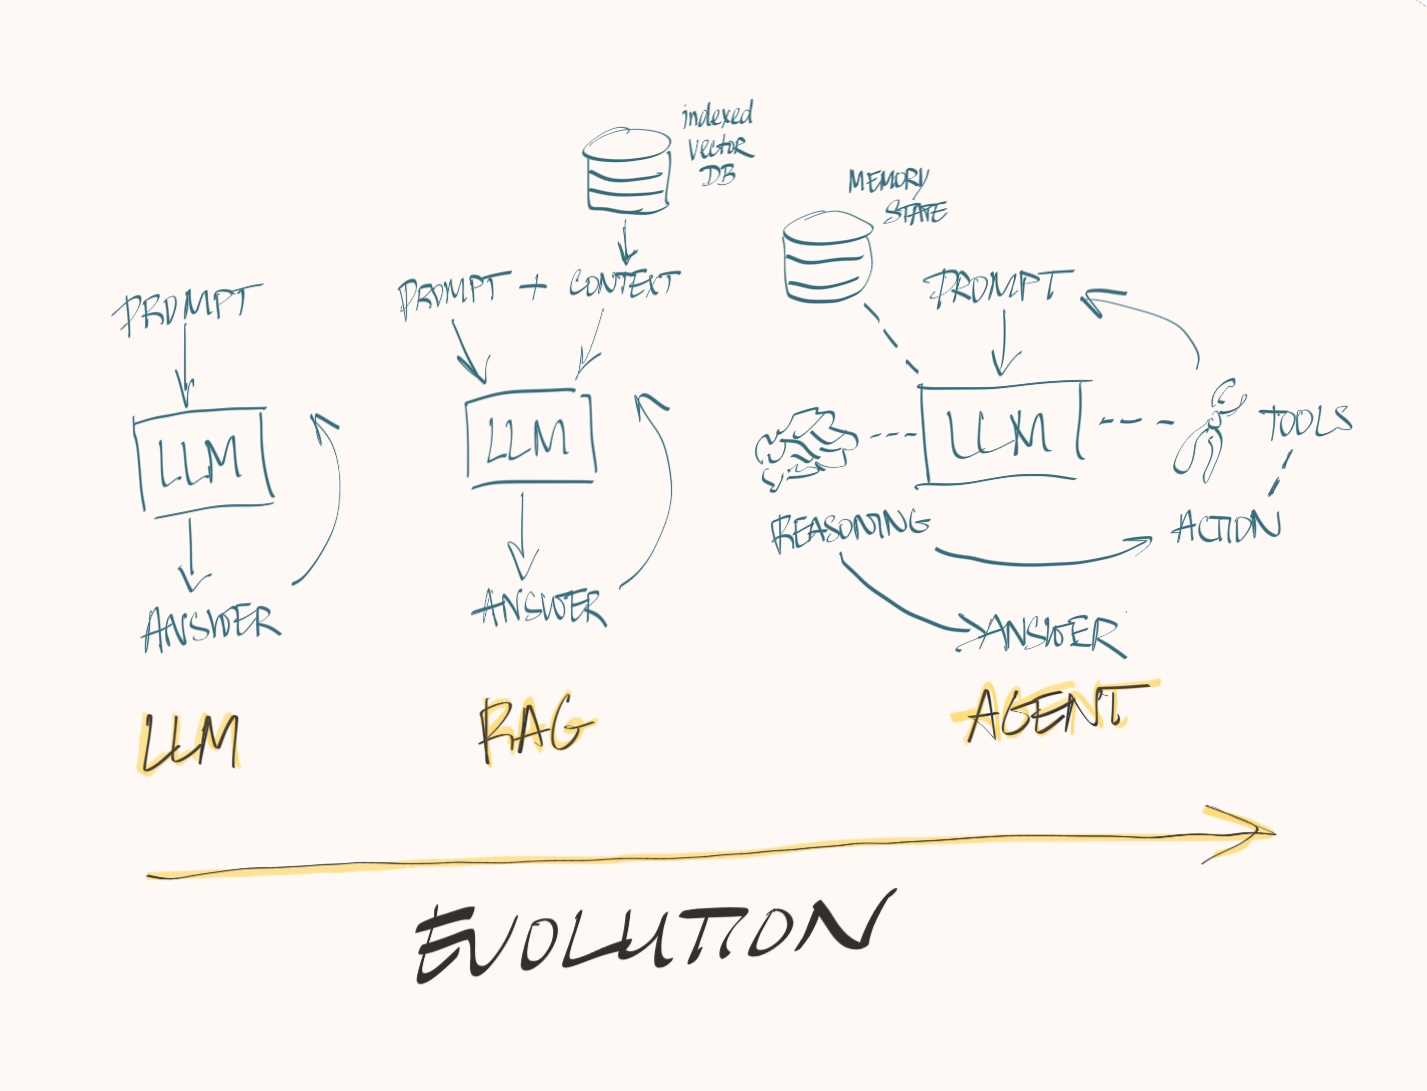
\includegraphics[width=\textwidth]{docs/llm_evolution.jpg}
    \caption{Evolution of LLM}
\end{figure}



\subsection{ZeroMQ for Local Communication}
\label{subsec:background:first_section:third_subsection}

Running several processes in parallel, namely a vision system, a voice recognizer, and a command execution of a LEGO train motor — requires communication. However, using Internet-based protocols like HTTP introduces latency and dependency. ZeroMQ is a lightweight messaging library that supports asynchronous communication between local processes without a central broker \cite{hintjens_zeromq_2013}. It supports flexible messaging patterns such as pub-sub and push-pull, which are ideal for small-scale distributed systems. ZeroMQ is frequently used in robotics and IoT applications for exactly this reason: it provides low-latency messaging and decouples components, increasing system robustness and fault tolerance \cite{wang_survey_2024, zhang-kennedy_systematic_2021}.


%
% Section: Der Zweite Abschnitt
%

\section{Related Work}
\label{sec:background:second_section} 

In this section we will give an overview of related works. For this we conducted an preliminary intensive literature research with the help of elicit, to be found in the appendix. We consulted it and derived most relevant sources. We will discuss this in detail in \ref{sec:background:second_section:first_subsection} 

Many research efforts have tackled similar challenges, such as running intelligent agents on edge devices, enabling offline control systems, and integrating LLMs with hardware. This section presents both academic work and open source frameworks reviewed to make a inform to realise the goal of this project.

% -------------------------------------------------
\subsection{Overview of Agentic Frameworks}
\label{subsec:background:first_section:first_subsection}

\begin{description} 
\item[\cite{yao_react_2023}]
This paper presents \textbf{ReAct}, a method for combining reasoning and actions inside LLMs. Instead of just generating answers, the model thinks through steps and takes actions in between. This structure makes it more reliable and interpretable. It worked really well in tasks like answering complex questions or navigating websites. I found this idea very useful as it shows how agentic behavior can be achieved without needing lots of training or hardware.

\item[\cite{asai_self-rag_2023}]
In this work, the authors introduce \textbf{Self-RAG}, which builds on retrieval-augmented generation by adding self-reflection. Basically, the model reflects on what it retrieved and decides if the info is useful before answering. This was tested on various question-answering and fact-checking tasks, and it outperformed other methods. This idea is interesting for edge cases, where every response needs to be more accurate because of limited retries.

\item[\cite{xi_rise_2023}]
This survey gives a very broad \textbf{overview of LLM-based agents,} from their design to how they can work together in groups. It even talks about things like social behavior in agent societies. I liked that it broke agents down into brain, perception, and action components. It helped me understand where my train control system fits into this bigger picture. They also discuss challenges with evaluation and generalization, which was helpful when deciding on a framework.

\item[\cite{jeong_adaptive-rag_2024}]
Jeong et al. suggest using a classifier to predict how hard a question is, and then select the right retrieval strategy. So the system doesn't waste resources on easy queries, and still handles harder ones properly. I think this is a smart way to optimize performance, especially when running locally. It avoids the “one size fits all” approach and adapts based on what’s needed.

\item[\cite{yan_corrective_2024}]
This paper focuses on improving what happens when document retrieval fails. The authors propose \textbf{CRAG}, a setup where the model can judge the quality of the retrieved data, and take action to fix it, like re-querying or using broader search. It also filters irrelevant info from the retrieved documents. This seems really helpful for systems that work offline or have limited memory, where the first retrieval might be bad.

\item[\cite{li_review_2024}]
Li's paper gives an \textbf{overview of three common agent techniques}: using tools, planning steps, and learning from feedback. What I found most useful was the idea of breaking systems into reusable modules (called LMPCs). It made me think more carefully about building the AI agent as components that can be reused later, like the voice input or the logic for stopping the train.

\item[\cite{paramanayakam_less_2024}]
The authors suggest that giving too many tools to a language model is inefficient. So, they propose a \textbf{smart tool selection method} that only shows the model a few tools at a time. This saves energy and time — they saw big improvements in speed and power use. I thought this paper supported the idea that it's okay to limit features if you can make smarter choices.

\item[\cite{dong_generalizing_2024}]
This paper combines an \textbf{LLM with a driving model} by letting the LLM make occasional high-level decisions, while a simpler model drives the car. It's like splitting the brain and the reflexes. This saves compute and works better in real-time. Even though this was about cars, I saw a lot of overlap with how I structured the train controller, where the LLM just decides what to do, but doesn’t touch the motor directly.

\item[\cite{huang_efficient_2024}]
Here, the authors built a system where \textbf{multiple units with LLMs} explain what’s happening on the road, in real time. Each unit uses environment and movement data to describe and reason about events. It was cool to see how they used prompt engineering to get better behavior without changing the model. This gave me ideas on how to handle narration or error feedback in my own project.

\item[\cite{tang_autoagent_2025}]
\textbf{AutoAgent} is a very advanced system that lets you build agents using just natural language. It comes with its own file manager, tool engine, and logic planner. The downside is that it's really resource-hungry. While it was impressive, I realized quickly it wouldn't fit on a Raspberry Pi. Still, I used it as a reference for what kinds of features matter when designing smaller agents.

\item[\cite{kumari_smolagents_2025}]
Kumari \textbf{compares LangGraph and SmolAgents}. SmolAgents is super lightweight and good for Pi-like setups but doesn’t support memory or planning. LangGraph supports branching and memory, but is a bit heavier. I agree with the conclusion: LangGraph is better if you want structure and flexibility, especially for projects like mine where logic and reactions matter.
\end{description}

%\begin{landscape}
    \begin{table}[htbp]
    \centering
    \caption{Comparison of Selected Agentic LLM Frameworks for Edge Deployment}
    \label{tab:framework_comparison}
    \resizebox{\textwidth}{!}{%
    \begin{tabular}{|l|l|c|c|c|l|l|l|}
        \hline
        \textbf{Framework} & \textbf{Architecture Type} & \textbf{Tool Use} & \textbf{Open Source} & \textbf{Edge-Ready} & \textbf{Workflow Support} & \textbf{Optimization} & \textbf{Limitations} \\
        \hline
        LangGraph & Graph-based workflows & Yes & Yes & Partial & Conditional branching, persistent memory & Modular Python design & Not pre-optimized for Pi; requires tuning \\
       
        SmolAgents & Minimalist agent & Yes & Yes & Yes & Linear (no memory/planning) & Extremely low resource usage & Lacks advanced decision-making and context retention \\
        
        AutoAgent & Zero-code agent OS & Yes & Yes & No & Full planning and memory & Rich features, but heavy runtime & Too resource-intensive for Raspberry Pi \\
        
        TinyAgent & Quantized tool caller & Yes & Partial & Partial (e.g., tested on higher-end devices) & None (only basic function calls) & 4-bit quantization for speed & No structured workflow or memory support \\
        
        Promp-tAI & LLM deployment infrastructure & No & Yes & Yes & None & Docker-based, optimized for inference & Does not offer agent logic or planning \\
        \hline
    \end{tabular}%
    }
    \end{table}
%\end{landscape}


% -------------------------------------------------
\subsection{Five Promising Frameworks}
\label{subsec:background:second_section:second_subsection}

\subsubsection{Top Frameworks in Detail}

\paragraph{LangGraph.} This framework allows agents to be defined as a graph of actions, memory updates, or tool calls. It supports branching logic and tool orchestration while maintaining a small enough footprint to potentially run on a Pi, especially when paired with quantized LLMs \cite{langchain_agent_2024, kumari_smolagents_2025}.

\paragraph{SmolAgents.} Designed for extremely low-resource environments, SmolAgents use minimal logic and quick tool calls. However, they lack long-term memory and planning capabilities, limiting their usefulness for complex tasks \cite{kumari_smolagents_2025, xi_rise_2023}.

\paragraph{AutoAgent.} A powerful, no-code environment for developing and deploying multi-agent workflows. It includes memory, file systems, and planning logic, but is too resource-heavy for embedded devices \cite{tang_autoagent_2025}.

\paragraph{TinyAgent.} A lightweight function-calling agent using 4-bit quantized models. Though efficient and responsive, it does not support memory, and limited public information makes integration difficult \cite{erdogan2024tinyagent}.

\paragraph{Promp-tAI.} A tool designed to deploy LLMs on edge devices using containerization. While helpful for infrastructure, it lacks agentic features like decision-making or tool use \cite{nezami2024promptai}.


% -------------------------------------------------
\subsubsection{ASR and Vision for Embedded AI}

Offline ASR on the Pi can be achieved using Vosk, which supports real-time speech-to-text without internet access \cite{vosk2023api}. For visual perception, lightweight models like YOLOv5 Nano and TensorFlow Lite enable object detection with 5–10 FPS on the Raspberry Pi \cite{lin2022realtime, tan2023lightweightcv}.


% -------------------------------------------------
\subsubsection{Educational Robotics and Constructivism}

This project continues previous student work at Hochschule Darmstadt using LEGO and Raspberry Pi platforms. While earlier versions relied on simple color sensors and MQTT-based control, this study introduces AI-based autonomy. The pedagogical foundation follows Papert's constructivist theory \cite{papert1980mindstorms}, where learning occurs through creation and experimentation. Related literature supports robotics as a powerful tool for fostering creativity and digital fluency in educational contexts \cite{resnick2009kindergarten,bers2020coding}.

% -------------------------------------------------
\subsection{Identified Gaps and Framework Justification}

Many frameworks either lack flexibility or are too demanding for embedded systems. SmolAgents is easy to deploy but too basic. AutoAgent supports complex agents but requires more memory than the Pi can provide. TinyAgent is fast but lacks planning. Promp-tAI assists with deployment but has no logic layer.

LangGraph stands out for its support of memory, conditional logic, and modular tools. It is also written in Python and designed to be extensible. When used with lightweight LLMs, LangGraph provides a practical foundation for building a responsive, voice- and vision-enabled train control agent on a Raspberry Pi.

% -------------------------------------------------
\section{Research Questions and Study Significance}
\label{sec:background:third_subsection:researchquestions}

After reviewing existing work on embedded AI systems and agentic LLM architectures, this study is guided by the following research questions, each rooted in the constraints and requirements of our real-world LEGO train system.
\begin{description}
    \item[RQ1:] \textit{How can agentic LLMs be deployed on resource-limited devices like the Raspberry Pi while still providing reliable performance for real-time control tasks?}\\
    
    Running an LLM on a Raspberry Pi locally presents clear challenges: low RAM, no GPU, and limited CPU power. This question investigates whether techniques such as quantization \cite{dettmers2022optimizers}, pruning \cite{han2016deep}, or the use of smaller open-source models (e.g., LLaMA variants) can support agentic behavior locally. In our setup, we use a quantized Ollama llama3-groq-tool-use model that can handle voice commands and make control decisions without cloud assistance. The agent must respond immediately, e.g., to stop the train if an obstacle appears on the track. Therefore, the inference time must be less than 1 to 3 seconds to be useful. The question is not just "can it run?" but "can it run fast enough to be useful?"
    
    \item[RQ2:] \textit{What communication architecture supports real-time coordination between an AI agent, object detection, and train motor control on a single edge device?} \\
    
    Instead of relying on frameworks like ROS or MQTT, this project uses ZeroMQ for its lightweight, brokerless decentralized design \cite{hintjens2013zeromq,zhang2021zeromqiot}. Components like the ASR module, the object detection process, and the train motor controller run in separately and communicate asynchronously using pub-sub patterns. This avoids blocking issues and allows the system participants to remain responsive even if one module slows down. The communication layer plays a critical role in making sure that decisions are made and executed reliably and in order, especially when reacting to safety-critical events.

    \item[RQ3:] \textit{How can simple but effective safety logic be implemented in a low-resource, autonomous control system?} \\
    
    Rather than complex reinforcement learning or advanced anomaly detection, our system focuses on lightweight, rule-based safety mechanisms. For example, the object detection module triggers a stop signal if an object is within a predefined proximity threshold. The LLM agent also considers recent context (via LangGraph memory) to prevent repeated or unsafe actions. Although there are more advanced safety techniques, this question looks at what can be achieved with limited compute and basic vision tools such as YOLOv5 Nano or TensorFlow Lite \cite{lin2022realtime,tan2023lightweightcv}.
\end{description}


%-------------------------------
\subsubsection{Study Significance}
\label{sec:background:third_subsection:study_significance}

To best of our knowledge this project offers a practical example of how to build a local, private, and low-cost intelligent control system; something that is still underexplored in real-world educational or prototyping contexts. The main value lies in how accessible and flexible the system is.

\begin{itemize}
  \item \textbf{Replicable:} It uses common hardware (Raspberry Pi, LEGO, USB mic), and all software is open-source.
  \item \textbf{Modular:} Components are separate and can be improved or replaced without rewriting the entire system.
  \item \textbf{Privacy-respecting:} No internet or cloud services are not required, which is valuable for school projects or sensitive environments.
  \item \textbf{Educational:} Students can explore Python coding, agent logic, voice control, asynchronous networking and safety protocols in one system.
  \item \textbf{Constructivist:} Based on hands-on experimentation and modular tinkering, the system aligns well with project-based learning approaches \cite{papert1980mindstorms,resnick2009kindergarten}.
\end{itemize}

By combining LLM reasoning, real-time inputs, and local tool control, the prototype creates opportunities for both exploration and practical deployment in constrained settings.


%\chapter{System Design and Architecture}
\label{ch:system_design}
\graffito{Note: High-level diagrams, component responsibilities, data flow but be created.}

outlines the system design of our proposed solution.

The architecture of the our proposed solution comprises several essential components to create an integrated and responsive system:

\begin{description}
    \item[LEGO Train Control Server] A dedicated Python application manages the actual train operations. The server receives command requests from the AI agent or the GUI controller over ZMQ, allowing it to directly execute actions such as start, stop, and speed adjustments. It also broadcasts the current train status to both controllers, enabling every participant of the system to be aware of the current status.
    
    \item[Graphical User Interface Controller] This application, which is also running on the Rapeberry Pi, allows users to control the train. It provides a video stream to the user and performs real-time object detection using computer vision under the hood. It communicates with the AI agent to ensure safe train operation, especially in cases where stopping the train is necessary to avoid collisions.
    
    \item[AI Agent] Built using Langgraph framework, this agent processes user inputs and translates them into command requests for the Lego train. Leveraging locally running LLM, it reasons through both user and system prompts and autonomously handles interactions by calling custom tools. The obstacle detection message sent by the GUI prompts the agent to halt the train and alert the user.
    
    \item[ZeroMQ Communication] Utilizing ZeroMQ facilitates fast, low-latency communication between components without requiring internet connectivity, ensuring reliable control over the LEGO train operation Alabed et al. (2023).
\end{description}


AI Agent: 
% Automatic Speech Recognition (ASR): Integrating ASR allows users to issue voice commands, thereby offering a hands-free control mechanism for the LEGO train. Utilizing open-source ASR libraries helps provide flexibility and affordability for implementation.}

 This agent leverages LangGraph's capabilities to gather and process various information streams, allowing it to understand user commands and respond appropriately. Its reasoning capacity enables it to make decisions based on the current state of the LEGO train system and the user suggested commands. 

 Running locally on the Raspberry Pi, the open-source LLM processes textual input and generates natural language responses. This enhances user interaction by enabling nuanced discussions and clarifying commands.

 
 State Management: The agent maintains a comprehensive awareness of the operational status of the train - whether it is moving, stopped, or facing any obstructions. By continuously monitoring the feedback from the train, the agent ensures prompt adjustments to its commands, enhancing the overall safety and reliability of operations.

 ZeroMQ Communication Protocol: Utilizing ZeroMQ enables effective and low-latency communication between the LangGraph AI agent, LEGO train control server and graphical user interface components. This is essential for real-time responsiveness, especially when dealing with external commands and emergency stops triggered by object detection.

%
% Section: Implementation
%
\section{Implementation}
\label{sec:system_design:implementation}
\graffito{Note: Languages, frameworks, libraries, algorithms used; software engineering details.}

\subsection{Methodology}

1. Local Deployment of LLMs
The implementation of locally running LLMs on the Raspberry Pi enhances data privacy and reduces latency, a critical factor for real-time applications like controlling a Lego train. Local deployment allows for quick processing of user queries and seamless integration with the ReAct agent without external dependencies.

2. Speech Recognition Integration
Incorporating ASR enables users to interact with the train through voice commands, providing flexibility to control operations hands-free. The system will leverage existing ASR solutions that can be integrated into Python environments, such as Vosk or Google’s Speech-to-Text, to parse voice commands into executable actions (Qiu et al., 2024).

3. Safety Protocols
Safety features are crucial, particularly in environments with moving trains. The User Interface Controller implements real-time object detection using frameworks like OpenCV and TensorFlow, analyzing video frames to identify obstacles. If an object is detected on the train track, the UI Controller signals the ReAct Agent to issue a stop command to the train control server, ensuring safe operation (Raisch & Krakowski, 2020).

4. Train Control Logic
The train control logic encapsulated in the Train Control Server interprets commands from both the ReAct agent and User Interface Controller, managing train status updates and broadcasting this information back over ZMQ. This ensures both control units have up-to-date information about the train's current state, providing an autonomous operational environment (Spitale et al., 2023).


\subsection{Implementation Plan}
Setting Up Raspberry Pi Environment: Install necessary software libraries, including LangGraph, ASR tools, and ZMQ.

2. Developing the AI ReAct Agent: Create functionality for the agent to process user inputs, augmented through LangGraph’s reasoning capabilities.

3. Integrating Train Control Server: Program train control logic, ensuring it effectively communicates with the ReAct agent and UI Controller.

4. Implementing Real-time Detection: Develop the object detection module, setting thresholds for distance and speed needed to trigger emergency commands.

5. Testing and Iteration: Conduct tests in real-time scenarios to refine interactions, safety features, and communication reliability.



The implementation process consists of the following steps:

1. Setting Up the Raspberry Pi: Establish a Raspberry Pi environment equipped with necessary libraries, including LangGraph, %ASR modules, 
ZMQ, and the open-source LLM.

2. Developing the RAG ReAct Framework: Create functions within the LangGraph RAG framework to interpret user inputs and translate them into corresponding commands for the LEGO train. This includes natural language understanding, state awareness, and decision-making logic.

3. Integrating Speech Recognition: Implement ASR capabilities to recognize voice commands issued by the user. This involves setting up and training the model to ensure it accurately interprets commands related to the operation of the train.

4. Testing Control Logic: Establish the control server logic for the LEGO train, which will handle commands from both the ReAct agent and the user interface. This server will continuously monitor the actions of the train and report its status to the agent in real time.

5. Implementing Safety Measures: To ensure safety during operation, the agent must react to disturbances in its environment, such as unexpected objects on the track. The system incorporates an object detection framework that triggers an emergency stop command when an obstacle is detected.


\subsection{Used Technology}

Langgraph ReAct Template

ollama with enhanced tool calling model

zmqt

OpenCv and Tensorflow with pretrained COCO



This framework and implementation model for train control assistant tool illustrate the multifaceted advantages of using LangGraph with locally operating LLMs, thus enhancing both the practical application and the theoretical foundations of advanced AI in resource restricted edge device contexts.

%
% Section: Evaluation
%
\section{Evaluation}
\label{sec:system_design:evaluation}
\graffito{Note: Test setup, metrics, baselines, tools (e.g., benchmarking framework, dataset splits).}


%
% Section: Results and Analysis Diskussion der Ergebnisse
%
\section{Results and Analysis}
\label{sec:system_design:results}
\graffito{Note: Plots, tables, runtime comparisons, accuracy, etc.}

The proposed AI ReAct Agent based on LangGraph, operating on a Raspberry Pi with LLMs, presents an innovative solution for autonomous control of a Lego train. By facilitating both text and voice commands, along with built-in safety protocols for real-time object detection, the system aims to deliver an efficient and reliable operational environment. Future work will focus on expanding the capabilities of the agent, including more complex decision-making processes and the potential for learning from environmental interactions.

Advantages of the Proposed System

The proposed LangGraph RAG ReAct agent on the Raspberry Pi provides several notable advantages:

- Enhanced Reasoning Capability: The integration of the LangGraph RAG framework allows the agent to reason through commands, offering intelligent responses that go beyond simple command execution. It can understand context and history of prior interactions, improving the overall user experience.

- State Management and Safety: The agent's ability to keep track of the train's operational state enhances safety and operational efficiency. This capability allows for dynamic adjustments based on both user commands and real-time environmental conditions.

- Accessibility: The ASR and LLM combination makes the system accessible to a broader audience, enabling users with varying levels of technical expertise to interact with the LEGO train system easily and intuitively.

- Cost-effective and Open-Source: The use of Raspberry Pi as the central platform alongside open-source tools lowers the overall cost barrier for development and implementation. This encourages experimentation and customization within educational and hobbyist communities.

\section{Methodology}
\label{sec:methodology}

This section outlines the full system architecture and implementation strategy behind the autonomous LEGO train prototype. The aim was to build a decentralized, modular, and voice-interactive control system driven by a local agentic LLM. Built entirely on a Raspberry Pi without cloud dependencies, the system integrates LangGraph, ZeroMQ, and lightweight ASR and vision tools to ensure autonomous behavior and safety.

\subsection{System Overview}

The architecture is composed of five main modules:

\begin{itemize}
    \item \textbf{LangGraph-based Agent:} interprets voice/text commands and executes tool functions.
    \item \textbf{Train Control Server:} interfaces with LEGO motor hardware.
    \item \textbf{UI Controller:} handles object detection, real-time feedback, and safety triggers.
    \item \textbf{ZeroMQ Network Layer:} manages asynchronous message passing across modules.
    \item \textbf{ASR Listener:} processes local speech commands using Vosk.
\end{itemize}

\begin{figure}[H]
    \centering
    \includegraphics[width=\textwidth]{langgraph-flow.png}
    \caption{LangGraph agent state transition loop (adapted from \texttt{langgraph.ai})}
\end{figure}

\subsection{LangGraph-Based AI Agent}

The LangGraph framework was chosen for its modular, reactive architecture. Unlike monolithic agents, LangGraph encodes tool execution and decision-making into a visualizable graph. Nodes represent either LLM reasoning steps or tool invocations; transitions are conditional.

\begin{lstlisting}[language=Python, caption=LangGraph reasoning node setup]
builder = StateGraph(State, input=InputState, config_schema=Configuration)
builder.add_node("call_model", call_model)
builder.add_node("tools", ToolNode(TOOLS))
builder.add_edge("__start__", "call_model")
builder.add_conditional_edges("call_model", route_model_output)
builder.add_edge("tools", "call_model")
\end{lstlisting}

The agent is responsible for interpreting user commands and invoking appropriate tools, all within a cycle of LLM reasoning and external execution.

\subsection{Train Control Server}

This server directly controls the LEGO motor using Build HAT. It uses the ZeroMQ \texttt{ROUTER} pattern to accept commands and the \texttt{PUB} pattern to broadcast updated statuses.

\begin{lstlisting}[language=Python, caption=Motor control interface]
def start(self, speed, direction):
    self.speed = speed if direction == "forward" else -speed
    self.train.start(self.speed)

def stop(self):
    self.train.stop()
\end{lstlisting}

This server is always listening for command requests and emits updated status after every successful action.

\subsection{User Interface and Object Detection}

The UI provides camera-based visual feedback and emergency detection. Obstacle detection is wired directly into the UI loop using TensorFlow Lite or YOLOv5 Nano. Detection triggers an alert to the AI agent via ZeroMQ.

\begin{lstlisting}[language=Python, caption=Triggering alerts from UI]
if detected_object['confidence'] > 0.6:
    send_alert("obstacle detected", detected_object)
\end{lstlisting}

This ensures the safety mechanism operates independently from the reasoning loop.

\subsection{ZeroMQ Messaging Layer}

ZeroMQ was selected due to its low-latency, modular, and broker-less design. The following patterns are used:

\begin{itemize}
    \item \textbf{DEALER/ROUTER:} for bi-directional commands between UI/Agent and the train controller
    \item \textbf{PUB/SUB:} for broadcasting train state to all components
\end{itemize}

\begin{lstlisting}[language=Python, caption=Socket setup]
dealer.setsockopt(zmq.HEARTBEAT_IVL, 2000)
dealer.setsockopt(zmq.RCVTIMEO, 30000)
sub.setsockopt_string(zmq.SUBSCRIBE, topic_filter)
\end{lstlisting}

\begin{figure}[H]
    \centering
    \includegraphics[width=\textwidth]{message-flow-architecture.png}
    \caption{ZeroMQ component messaging and socket topology}
\end{figure}

\subsection{Always-On ASR with Vosk}

Speech input is processed using Vosk for offline ASR. Wake word detection filters irrelevant audio, avoiding noisy LLM queries.

\begin{lstlisting}[language=Python, caption=Wake-word filtering]
if WAKE_WORD in result_text.get("text", ""):
    print("Wake word detected")  # Switch to command mode
\end{lstlisting}

Once active, transcribed commands are passed to the LangGraph entry node for further reasoning and tool invocation.

\subsection{Tool Functions and Runtime State Sync}

Agent tools encapsulate train commands like \texttt{start()}, \texttt{stop()}, \texttt{get\_status()}. Runtime state is maintained centrally.

\begin{lstlisting}[language=Python, caption=Train control tool call]
async def start(speed: int, direction: str) -> dict:
    result = await send_train_command("start", [speed, direction])
    return {"train_status": result}
\end{lstlisting}

The \texttt{RuntimeState} singleton synchronizes state between components, ensuring coherent execution even with asynchronous delays.

\subsection{Startup Pattern and Background Threads}

All side-effect logic is centralized in \texttt{startup.py}, including listener registration, ASR thread launch, and ZeroMQ init.

\begin{lstlisting}[language=Python, caption=Startup orchestration]
start_ui_listener()
start_asr_listener()
start_train_status_listener()
\end{lstlisting}

This clean design allows the agent logic to remain pure and testable, and simplifies shutdown and reinitialization.

\subsection{Educational Practices and Insights}

The codebase intentionally mirrors good modular software engineering principles to enhance its use in educational contexts. Each subsystem—ASR, UI, controller, LangGraph agent—is independently testable. Explicit comments and verbose logs were used for student understanding.

Suggested educational tasks:

\begin{itemize}
    \item Modify the \texttt{change\_speed()} tool to accept percentage deltas
    \item Add fallback rules to the LangGraph agent for offline error handling
    \item Profile latency for different ASR wake-word models
\end{itemize}

\section{Conclusion of Section}

This architecture prioritizes safety, modularity, and transparency while operating under embedded constraints. Though the implementation is incomplete in a few areas (e.g., advanced agent memory), it lays a solid foundation for future educational deployment and system scalability.

\chapter{Evaluation and Results}
\label{ch:evaluation}

This section presents the system’s performance observations, functional validation, and development insights derived during implementation. As this project integrates diverse asynchronous components under real-time constraints on limited hardware, both technical performance and practical engineering challenges are assessed.

\section{Evaluation Strategy}

The evaluation combined direct functionality tests, empirical performance observation, and developer-driven stress testing. Formal benchmarks were limited due to runtime variability on embedded hardware. Most system components were validated on macOS with mock objects and finalized on a Raspberry Pi 4 Model B.

\subsection{Performance Observations}

Agent response time was generally acceptable for command-level interaction. Commands sent to the LangGraph agent (via speech or GUI) triggered tool responses with average latency between 6 to 8 seconds. Notably:

\begin{itemize}
  \item **ASR + agent query roundtrip**: $\approx$ 6-8s
  \item **Agent tool execution**: $\approx$ 0.4–0.8s
  \item **Object detection loop (TFLite)**: 0.5s/frame
\end{itemize}

Background threading and event synchronization improved performance stability. However, early stages suffered from excessive polling, redundant feed refreshes, and unintended re-initialization of sockets.

\subsection{Functional Testing}

\begin{itemize}
  \item \textbf{Train Controller and UI:} Fully tested. Commands like \texttt{start}, \texttt{stop}, and \texttt{get\_status} executed reliably. UI responded to runtime status broadcasts.
  \item \textbf{Agent + ASR:} Wake-word filtering and command dispatch worked as designed. Real-time audio input via Vosk recognized short phrases with high accuracy under low-noise conditions.
  \item \textbf{Object Detection:} Operational via camera feed. Simulated obstacle triggers correctly stopped the train through UI-based alerts.
  \item \textbf{System Integration:} Full integration test on Raspberry Pi succeeded. The agent received requests from ASR and UI and dispatched correct ZeroMQ messages. However, frequent restarts were needed to clear socket issues in LangGraph.
\end{itemize}

\subsection{Challenges and Debugging Journey}

The development process was exploratory and iterative. The project involved first-time use of Python for system integration, LangGraph for agent design, and ZeroMQ for asynchronous messaging.

Key challenges included:

\begin{itemize}
  \item \textbf{Asynchronous complexity:} Thread coordination across modules was difficult to debug, especially due to LangGraph’s internal asyncio event loops.
  \item \textbf{LangGraph instabilities:} Some template examples were broken due to dependency mismatches. Workarounds were required to bypass version conflicts, particularly with the OllamaChat class initialization.
  \item \textbf{Cyclic imports and state injection:} It was not initially clear how to pass shared state or runtime values into LangGraph nodes. Non-graph members had no state access until centralized runtime structures were enforced.
  \item \textbf{Socket re-initialization:} LangGraph reloaded socket connections internally during startup. To resolve this, socket allocation was moved out of agent code and initialized centrally in \texttt{startup.py}.
\end{itemize}

Despite these barriers, the system now runs reliably when started via the unified entrypoint. Lessons learned from failures played a central role in achieving final integration.

\section{Summary}

The system meets the primary goal of demonstrating a locally deployed, agentic LLM-driven autonomous controller on embedded hardware. While several architectural workarounds were necessary, the resulting prototype achieves real-time voice-command response, tool-calling behavior, and object-reactive control. Most importantly, it offers a strong platform for education and further exploration.

\chapter{Conclusion and Future Work}
\label{ch:conclusion}

\section{Summary of Findings}

This study explored the feasibility and architecture of deploying agentic large language models (LLM) on edge devices, specifically a Raspberry Pi 4 to autonomously control a LEGO train. By integrating LangGraph, ZeroMQ, and locally hosted ASR and object detection modules, the project successfully demonstrated a modular off-line control system for real-time interaction with a physical environment.

The system achieved voice-controlled operation, obstacle-based emergency stopping, and modular extension through message-based coordination. Despite the limited compute environment, the agentic LLM managed to interpret commands, invoke tools, and synchronize state through a combination of design abstractions and lightweight frameworks.

\section{Contributions and Educational Value}

This work offers not only a functioning prototype but also a pedagogical foundation for teaching agentic AI and edge computing. It demonstrates:

\begin{itemize}
    \item The viability of LangGraph-based agents in constrained environments
    \item How ZeroMQ can structure local component communication in real-time robotics
    \item How tool-calling and runtime state sync support fault tolerance
    \item The value of modularity in project-based learning and debugging
\end{itemize}

As part of the KinderCampus program, this system is expected to serve as a learning artifact for students exploring AI, voice interfaces, and safe control mechanisms.

\subsection{Limitations}

Despite its success, the current system has limitations:

\begin{itemize}
    \item raspberry Pi 4, is too weak. Pi 5 with more RAM would be more suitable. 
    \item LangGraph’s memory and planning capabilities are not fully utilized
    \item The object detection pipeline is lightweight but still CPU-intensive for longer runs
    \item Debugging async Python workflows remains challenging without deep logging
\end{itemize}

In addition, LangGraph’s rapidly evolving API made consistent debugging difficult, especially when combined with unofficial community examples and partial documentation.

\section{Future Work}

Future improvements could include:

\begin{itemize}
    \item Implementing memory-aware agent behavior for better multi-turn interactions
    \item Integrating more efficient wake-word detection and noise-tolerant ASR modules
    \item Porting visual detection to edge-accelerated inference frameworks like Coral or Jetson
    \item Building agent fallback logic for better user experience during network uncertainty
    \item Formalizing agent behavior through testing suites (better prompting)
\end{itemize}

From an educational angle, new modules can be created for students to:
\begin{itemize}
    \item Design their own tools and link them into the agent graph
    \item Test socket-based communication between custom GUIs and hardware
    \item Simulate safety conditions and observe agent decisions
\end{itemize}

\section{Final Remarks}

Building autonomous, voice-enabled robotics on resource-limited hardware is complex—but increasingly accessible. The combination of open-source tools like LangGraph, Ollama, ZeroMQ, and TFLite allows for educational systems that bridge theory and practice. While the development journey was filled with technical detours, cyclic imports, and uncooperative package versions, it led to a working system with real-world potential and classroom utility. More importantly, it taught me invaluable lessons in modular design, state management, and human-AI interfaces.



In conclusion, the proposed structure and operational framework provide a reliable AI-driven solution for controlling physical devices while ensuring adaptability, efficiency, and safety measures in real time. The integration of a modular design across components proposes not only a robust framework for this specific task but can also serve as a model for future AI applications in robotics and beyond.



%*************************************************************************
% Recommendations
%*************************************************************************
%\part{Empfehlungen zur Erstellung wissenschaftlicher Abschlussarbeiten}
%\label{pt:recommendations}
%\include{chapters/recommendations/abstract}

%*************************************************************************
% Backmatter
%*************************************************************************
\appendix
%\renewcommand{\thechapter}{\alph{chapter}}
\cleardoublepage
%\part{Appendix}
%\appendix
\section*{Appendix Attachments: Original Source Document}
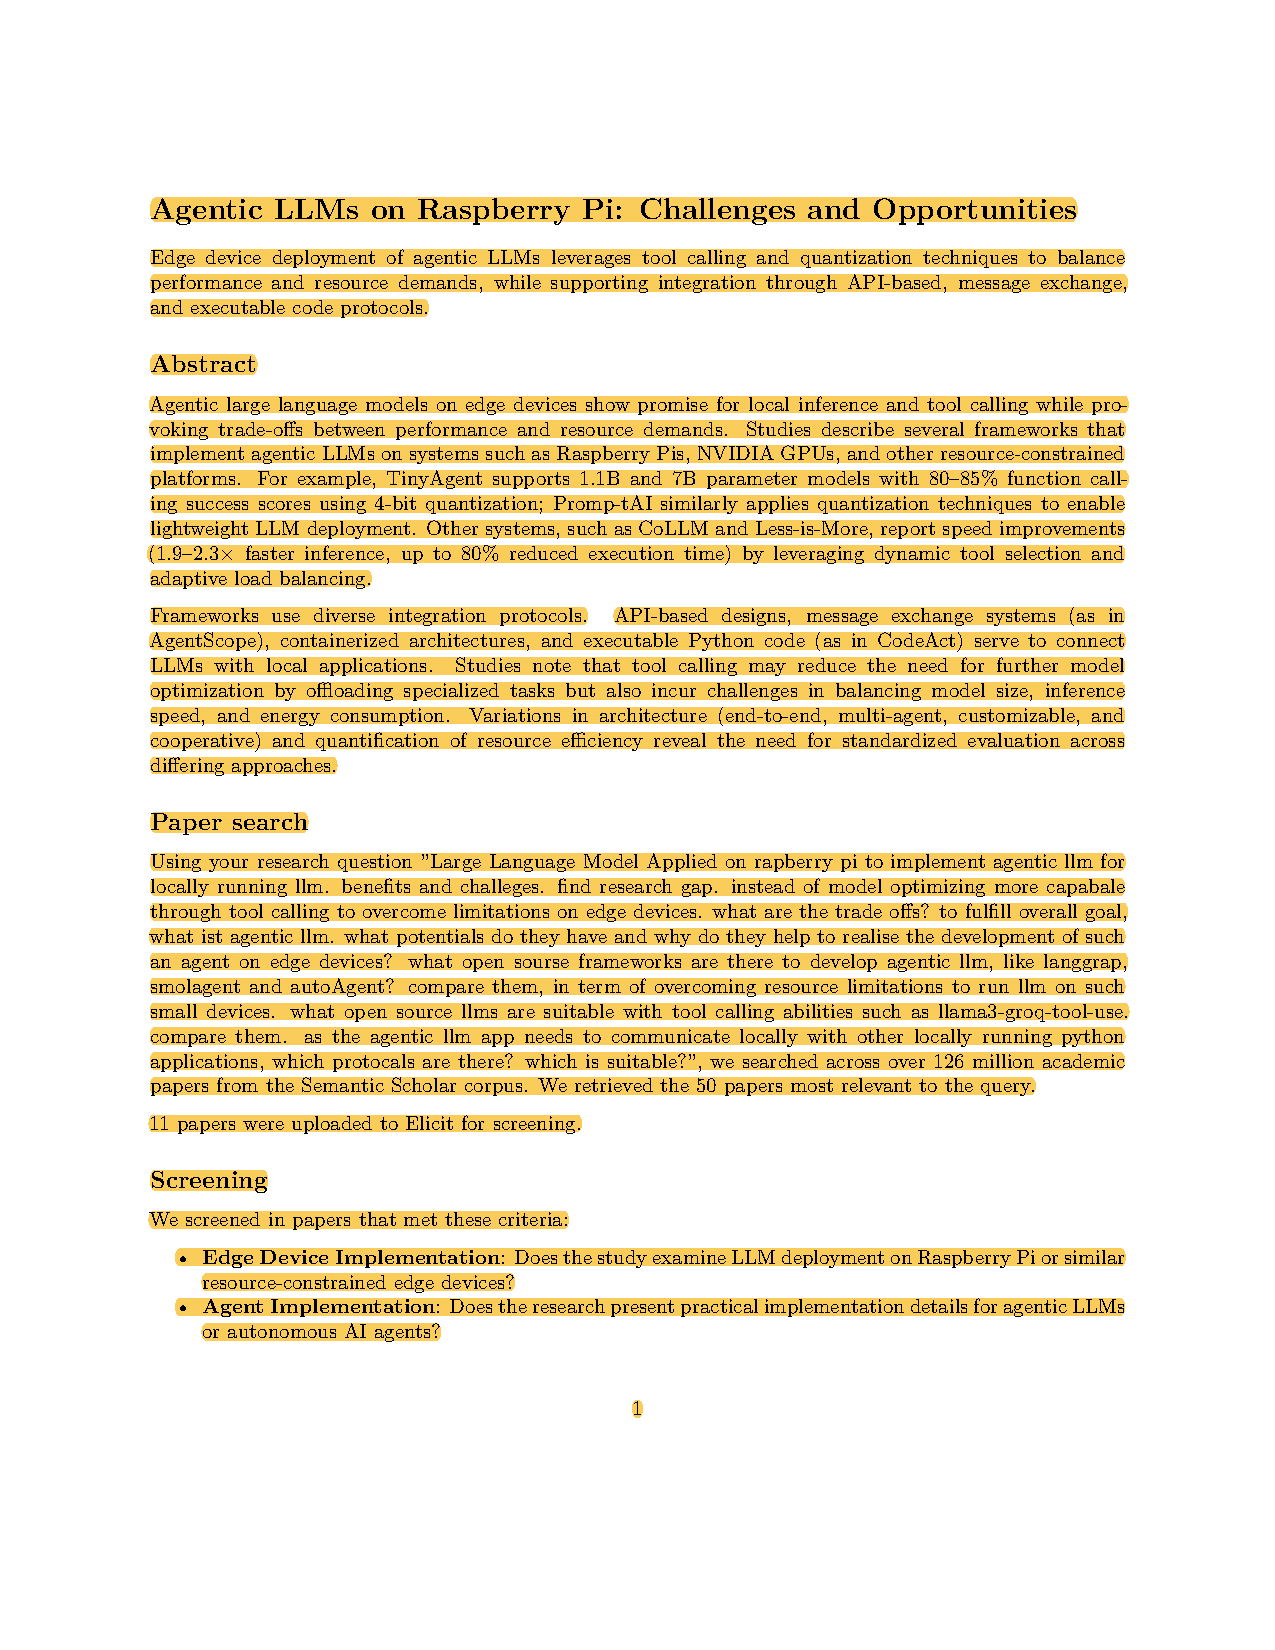
\includepdf[pages=-]{chapters/Attachments/Elicit.pdf}
%\include{chapters/examples/appendix01}
%\include{chapters/examples/appendix02}
%*************************************************************************
% Other Stuff in the Back
%*************************************************************************
\cleardoublepage\include{frontbackmatter/Bibliography}
%*************************************************************************
% Game Over: Restore, Restart, or Quit?
%*************************************************************************
\end{document}
%*************************************************************************
